\documentclass[conference]{IEEEtran}
\IEEEoverridecommandlockouts
\usepackage{amsmath,amssymb,amsfonts}
\usepackage{graphicx}
\usepackage{textcomp} 
\usepackage{xcolor}

\usepackage[utf8x]{inputenc}

\usepackage[english]{babel}
\usepackage{cite}               

\usepackage{tikz}
\usetikzlibrary{calc,trees,positioning,arrows,chains,shapes.geometric,%
    decorations.pathreplacing,decorations.pathmorphing,shapes,%
    matrix,plotmarks, shapes.symbols,arrows.meta}
%\usepackage{tkz-graph}
\usepackage{pgfplots}
\usepackage{pgffor}
\usepackage{circuitikz}
\usepackage{balance}
\usepgfplotslibrary{dateplot, groupplots}

\usepackage{amsmath}

\usepackage{enumerate}
\usepackage{mathtools}
\usepackage{algorithmic}
\usepackage{amssymb, amsthm}
\usepackage[]{algorithm2e}
\renewcommand{\algorithmicrequire}{\textbf{Input:}}
\renewcommand{\algorithmicensure}{\textbf{Output:}}
\usepackage{gnuplot-lua-tikz}
%\usepackage{subfigure}

\usepackage{pgfplots}
%\usepackage{pgfplotstable}
\usetikzlibrary{matrix,arrows,decorations.pathmorphing}

\newcommand{\orif}[1]{\textcolor{green}{[#1 -- ORI-FIXED]}}
\newcommand{\ori}[1]{\textcolor{red}{[#1 -- ORI]}}
\newcommand{\arik}[1]{\textcolor{red}{[#1 -- ARIK]}}
\newcommand{\dor}[1]{\textcolor{purple}{[#1 -- DOR]}}
\newcommand{\dorf}[1]{\textcolor{orange}{[#1 -- DOR-FIXED]}}

\newcommand{\forRevThree}[1]{{#1}}


\newcommand{\inblue}[1]{{#1}}

\newcommand{\inred}[1]{{#1}}


\def \myScale {0.82}

\newcommand{\ingreen}[1]{{#1}}

\newcommand\diag[4]{%
  \multicolumn{1}{p{#2}|}{\hskip-\tabcolsep
  $\vcenter{\begin{tikzpicture}[baseline=0,anchor=south west,inner sep=#1]
  \path[use as bounding box] (0,0) rectangle (#2+2\tabcolsep,\baselineskip);
  \node[minimum width={#2+2\tabcolsep-\pgflinewidth},
        minimum  height=\baselineskip+\extrarowheight-\pgflinewidth] (box) {};
  \draw[line cap=round] (box.north west) -- (box.south east);
  \node[anchor=south west] at (box.south west) {#3};
  \node[anchor=north east] at (box.north east) {#4};
 \end{tikzpicture}}$\hskip-\tabcolsep}}

\newtheorem{lemma}{Lemma}
%\newtheorem{proof}{Proof}
\newtheorem{theorem}{Theorem}

\makeatletter
%%%%%%%%%%%%%%%%%%%%%%%%%%%%%% User specified LaTeX commands.
%\def\ps@IEEEtitlepagestyle{%
%  \def\@oddfoot{\mycopyrightnotice}%
%  \def\@evenfoot{}%
%}
%\def\mycopyrightnotice{%
%  {\footnotesize ISBN 978-3-903176-39-3© 2021 IFIP\hfill}% <--- Change here
%  \gdef\mycopyrightnotice{}% just in case
%}

%%%%% FOR REVISION %%%%%%%

\usepackage{xcolor} 
\usepackage{url}
\usepackage{float}
\usepackage{color}
\usepackage{tikz}
\usepackage{verbatim}
\usepackage{fancyvrb}

\newcommand{\fixed}[1]{\vskip 4mm \noindent{\color{blue} \textbf{Response:} {#1}} \vskip 5mm}
%\newcommand{\notfixed}[1]{\todo[inline,linecolor=red,backgroundcolor=red!5,bordercolor=red]{ {\footnotesize NOT FIXED: {#1}}}}

%\newcommand \fixed[1]{{\noindent\color{blue}#1}}

\newcommand \reviewer[1]{{\noindent\color{black}#1}}


%\renewcommand \ori[1]{}
%\renewcommand \janos[1]{}

\newcommand{\hash}{\mathpzc{h}}
%\newcommand{\deth}{\mathpzc{k}}
\newcommand{\deth}{\hat{h}}

\usepackage{mdframed}
\newcommand{\citetext}[1]{\protect\begin{mdframed}[leftmargin=1cm,rightmargin=1cm,shadow=true,shadowcolor=black!20,shadowsize=4pt] {\footnotesize \color{black} #1 } \protect\end{mdframed}}

\usepackage{amsmath,amssymb,amsthm}

\usepackage{bbold}
\newcommand \prob{\mathbb{P}}
%%%%%%%%%%%%%%%%%%%%%%%%%%




\pgfplotsset{compat=1.16}
\begin{document}



%\title{Distributed Sketching with  Traffic-Aware Summaries}
\title{Compressing Distributed Network Sketches with  Traffic-Aware Summaries}
%\title{SKTC: Distributed Sketching with Lightweight Summaries}



\author{\IEEEauthorblockN{\large Dor Harris, Arik Rinberg and Ori Rottenstreich}}

% for page number
%\thispagestyle{plain}
%\pagestyle{plain}
%\thispagestyle{empty}
%\pagenumbering{gobble}

\maketitle
\pagestyle{plain}
%\begingroup\renewcommand\thefootnote{\textsection}
%\footnotetext{The first two authors contributed equally.}
%\endgroup



\begin{abstract}
Network measurements are important for identifying congestion, DDoS attacks, and more. To support real-time analytics, stream ingestion is performed jointly by multiple nodes, each observing part of the traffic, periodically reporting its measurements to a single centralized server that aggregates them. To avoid communication congestion, each node reports a compressed version of its collected measurements. Traditionally, nodes symmetrically report summaries of the same size computed on their data. We explain that to maximize the accuracy of the joint measurement, nodes should imply various compression ratios on their measurements based on the amount of traffic observed by each node. We illustrate the approach for three common sketches: The Count-Min sketch (CM), which estimates flow sizes as well as for the K-minimum-values (KMV) sketch and the HyperLogLog (HLL), which both estimate the number of distinct flows. For each sketch, we compute node compression ratios based on the traffic distribution. \inblue{In general, this is done with a single round of communication with the central server, after which the compression ratio for each node can be computed.}
We perform extensive simulations for the sketches and analytically show that, under real-world scenarios, our sketches send smaller summaries than traditional ones while retaining similar error bounds. 
%To this end, we propose the CM-SKTC sketch, and the KMV-SKTC sketch.
%The CM-SKTC sketch allows for arbitrary compression ratios. We describe a method of calculating compression ratios based on the traffic distribution to the ingestion nodes, which retain the overall error of the built sketch. These rations lead to a reduction of the amount of data sent over the network without sacrificing error. We analytically measure the accuracy and performance of CM-SKTC.
%and conduct experiment to measure them under multiple scenarios. We show that CM-SKTC allows a reduction of up to $10\%$ in network communication while retaining the error bounds of existing compression methods. Realistic evaluation shows a similar reduction to the theoretical case.
%We then present the KMV-SKTC sketch and present the amount of data it sends over the network. We show that the KMV-SKTC sketch sends a constant amount of data, as opposed to a linear amount in the number of ingestion nodes. We then analyze its accuracy and performance, and conduct similar experiments.
\end{abstract}

\begin{IEEEkeywords}
Measurement,  Computer network management %Network Algorithms %Distributed Sketching
\end{IEEEkeywords}

{\let\thefootnote\relax\footnotetext{
%A preliminary version of this article appears at 
%IFIP Networking, Virtual Conference, June 2021~\cite{IFIP21}. This submission includes the following new technical contributions:


%$\bullet$ The Proofs for Lemma 1 and Theorems 1-2. Lemma 2 and its proof are also first presented here.

%$\bullet$ An extension of the traffic aware-approach to the HyperLogLog sketch (Subsection II.C and Section VI are new). New experimental results for this sketch appear in the new Subsection VII.E.   

Dor Harris, Arik Rinberg and Ori Rottenstreich are with the Technion, Haifa, Israel. (Emails: dorharris@cs.technion.ac.il, arikrinberg@campus.technion.ac.il, or@technion.ac.il). 
The first two authors contributed equally. A preliminary version of this article \inred{appeared} at IFIP Networking, Virtual Conference, June 2021~\cite{IFIP21}.
}
}
%\makeatother



\section{Introduction}\label{sktc-sec:intro}
Network designers need to gather analytics about the performance of the network to better understand what is happening behind the curtain. 
\ingreen{These are useful for traffic engineering, 
for reaching a higher utilization of the infrastructure,
for reducing link congestion, and for detecting anomalies when they happen.} Switches generally do not have sufficient memory to hold entire measurement models for large data streams, therefore the network designer generally sacrifices accuracy for a lower memory footprint.
Data sketching algorithms, or \textit{sketches} for short \cite{cormode2012synopses}, are
an indispensable tool for such high-speed low-memory-footprint computations. Sketches  estimate some function
of a large stream \ingreen{such as} \inblue{flow sizes}~\cite{CountMin} (i.e., the number of packets in a flow), \inblue{stream cardinality}~\cite{datar2002comparing, flajolet1983probabilistic} (i.e., the number of flows in a stream), the top-$k$ most common items~\cite{metwally2005efficient} or  frequency changes~\cite{IMCBal03}.
They are supported by many data analytics platforms such as PowerDrill~\cite{heule2013hyperloglog},
Druid~\cite{druid}, Hillview~\cite{hillview}, and Presto~\cite{presto} as well as \ingreen{by} standalone toolkits~\cite{apache-datasketches}.


Measurements are conducted in switches  all over the network; however, to successfully analyze network behavior, measurement data needs to be gathered in a centralized server that can see \ingreen{a wider view}.
\forRevThree{A stream of multiple flows passes through the network, with disjoint parts of the stream sampled by multiple \emph{ingestion nodes}, where parts of the same flow may be ingested by different nodes. The ingestion nodes periodically propagate their local sketch to a \emph{central node}, as illustrated in Figure~\ref{sktc-fig:ingestion-nodes}.  The network has to handle the trade-off of sending data packets vs. sending crucial control packets with sketch information~\cite{zhang2010optimizing, %zhang2009spatio,
benson2010understanding}. A way to reduce these control packets is by compressing the sketches before transferring them to a central analytics node.}



%\inred{To capture this behavior, we treat all of the incoming packets to the network as originating from a single \emph{stream}, which consists of multiple \emph{flows}.}
%\inblue{The stream is split into disjoint parts observed by multiple \emph{ingestion nodes}. Parts of the same flow may be ingested by different nodes.}  Once the nodes have a sketch ready to be sent (e.g., they periodically receive a packet signaling the end of their current stream and start a new one) they propagate their local sketch to a \emph{central node}~\cite{huang2017sketchvisor, li2016flowradar, liu2016one}. This is illustrated in Figure~\ref{sktc-fig:ingestion-nodes}. The network has to handle the trade-off of sending data packets vs. sending crucial control packets~\cite{zhang2010optimizing, %zhang2009spatio,
%benson2010understanding} with sketch information. A way to reduce these control packets is by compressing the sketches before transferring them to a central analytics node. 

\inblue{Compressing is crucial as network managers may have many sketches estimating different measurements concurrently. While each sketch alone may be insignificant, their aggregate is noticeable at the network level. Additionally, the sketch may be collecting measurements in low bandwidth networks~\cite{muthitacharoen2001low, margaritis2003peer}}, \ingreen{making the sketch size critical.}


\begin{figure}
    \centering
    %\includegraphics[width=0.9\linewidth]{figures/IngestionNodesPic.png}
    \tikzset{every picture/.style={line width=0.75pt}} %set default line width to 0.75pt    
    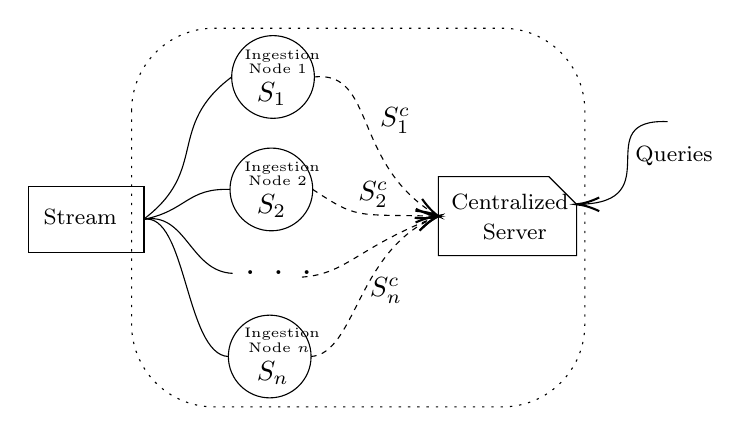
\begin{tikzpicture}[x=0.75pt,y=0.75pt,yscale=-1,xscale=1]
    %uncomment if require: \path (0,300); %set diagram left start at 0, and has height of 300
    
    %Shape: Rectangle [id:dp7800934124171983] 
    \draw   (117,155.65) -- (172.78,155.65) -- (172.78,187.53) -- (117,187.53) -- cycle ;
    %Shape: Ellipse [id:dp20814509523202052] 
    \draw   (215.02,103.05) .. controls (215.02,92.05) and (223.94,83.13) .. (234.94,83.13) .. controls (245.95,83.13) and (254.87,92.05) .. (254.87,103.05) .. controls (254.87,114.06) and (245.95,122.98) .. (234.94,122.98) .. controls (223.94,122.98) and (215.02,114.06) .. (215.02,103.05) -- cycle ;
    %Shape: Ellipse [id:dp5192677502317808] 
    \draw   (214.22,157.24) .. controls (214.22,146.24) and (223.14,137.32) .. (234.15,137.32) .. controls (245.15,137.32) and (254.07,146.24) .. (254.07,157.24) .. controls (254.07,168.25) and (245.15,177.17) .. (234.15,177.17) .. controls (223.14,177.17) and (214.22,168.25) .. (214.22,157.24) -- cycle ;
    %Shape: Circle [id:dp7676828342293531] 
    \draw   (213.43,237.73) .. controls (213.43,226.73) and (222.35,217.81) .. (233.35,217.81) .. controls (244.35,217.81) and (253.27,226.73) .. (253.27,237.73) .. controls (253.27,248.74) and (244.35,257.66) .. (233.35,257.66) .. controls (222.35,257.66) and (213.43,248.74) .. (213.43,237.73) -- cycle ;
    %Snip Single Corner Rect [id:dp7350487709437881] 
    \draw   (314.63,151.1) -- (367.87,151.1) -- (381.18,164.41) -- (381.18,189.12) -- (314.63,189.12) -- cycle ;
    %Curve Lines [id:da7243599111171348] 
    \draw   [dash pattern={on 2pt off 2pt}]   (254.87,103.05) .. controls (284.45,99.9) and (273.03,145.17) .. (313.4,169.38) ;
    \draw [shift={(314.63,170.11)}, rotate = 209.86] [color={rgb, 255:red, 0; green, 0; blue, 0 }  ][line width=0.75]    (10.93,-3.29) .. controls (6.95,-1.4) and (3.31,-0.3) .. (0,0) .. controls (3.31,0.3) and (6.95,1.4) .. (10.93,3.29)   ;
    %Curve Lines [id:da4335557046839309] 
    \draw   [dash pattern={on 2pt off 2pt}]   (254.07,157.24) .. controls (275.66,171.37) and (273.66,169.27) .. (312.82,170.07) ;
    \draw [shift={(314.63,170.11)}, rotate = 181.27] [color={rgb, 255:red, 0; green, 0; blue, 0 }  ][line width=0.75]    (10.93,-3.29) .. controls (6.95,-1.4) and (3.31,-0.3) .. (0,0) .. controls (3.31,0.3) and (6.95,1.4) .. (10.93,3.29)   ;
    %Curve Lines [id:da47273415849462186] 
    \draw   [dash pattern={on 2pt off 2pt}]   (253.27,237.73) .. controls (274.86,236.16) and (275.18,186.66) .. (312.89,170.81) ;
    \draw [shift={(314.63,170.11)}, rotate = 519.15] [color={rgb, 255:red, 0; green, 0; blue, 0 }  ][line width=0.75]    (10.93,-3.29) .. controls (6.95,-1.4) and (3.31,-0.3) .. (0,0) .. controls (3.31,0.3) and (6.95,1.4) .. (10.93,3.29)   ;
    %Curve Lines [id:da7986835200568454] 
    \draw   [dash pattern={on 2pt off 2pt}]   (248.89,199.48) .. controls (270.48,197.91) and (275.05,185.52) .. (312.88,170.78) ;
    \draw [shift={(314.63,170.11)}, rotate = 519.15] [color={rgb, 255:red, 0; green, 0; blue, 0 }  ][line width=0.75]    (10.93,-3.29) .. controls (6.95,-1.4) and (3.31,-0.3) .. (0,0) .. controls (3.31,0.3) and (6.95,1.4) .. (10.93,3.29)   ;
    %Rounded Rect [id:dp16891083296577403] 
    \draw  [dash pattern={on 0.84pt off 2.51pt}] 
    (166.81,119.26) .. controls (166.81,97.34) and (184.58,79.57) .. (206.49,79.57) -- (345.47,79.57) .. controls (367.39,79.57) and (385.16,97.34) .. (385.16,119.26) -- 
    %(166.81,113.26) .. controls (166.81,91.34) and (184.58,73.57) .. (206.49,73.57) -- (345.47,73.57) .. controls (367.39,73.57) and (385.16,91.34) .. (385.16,113.26) -- 
    %(385.16,232.31) .. controls (385.16,254.23) and (367.39,272) .. (345.47,272) -- (206.49,272) .. controls (184.58,272) and (166.81,254.23) .. (166.81,232.31) -- cycle ;
    (385.16,222.31) .. controls (385.16,244.23) and (367.39,262) .. (345.47,262) -- (206.49,262) .. controls (184.58,262) and (166.81,244.23) .. (166.81,222.31) -- cycle ;
    
    %Curve Lines [id:da7483451131891823] 
    \draw    (172.5,171.67) .. controls (204.38,147.76) and (183.14,126.96) .. (215.02,103.05) ;
    %Curve Lines [id:da3567735385248336] 
    \draw    (172.5,171.67) .. controls (193.22,167.68) and (193.5,156.45) .. (214.22,157.24) ;
    %Curve Lines [id:da8413889792937872] 
    \draw    (172.5,171.67) .. controls (193.22,167.68) and (194.78,196.87) .. (215.5,197.67) ;
    %Curve Lines [id:da820436037263437] 
    \draw    (172.5,171.67) .. controls (193.22,167.68) and (192.71,236.94) .. (213.43,237.73) ;
    %Curve Lines [id:da6059682612620094] 
    \draw    (425.01,124.57) .. controls (386.35,122.99) and (426.58,163.59) .. (382.54,164.39) ;
    \draw [shift={(381.18,164.41)}, rotate = 360.01] [color={rgb, 255:red, 0; green, 0; blue, 0 }  ][line width=0.75]    (10.93,-3.29) .. controls (6.95,-1.4) and (3.31,-0.3) .. (0,0) .. controls (3.31,0.3) and (6.95,1.4) .. (10.93,3.29)   ;
    
    % Text Node
    \draw (123.1,165.49) node [anchor=north west][inner sep=0.75pt]  [font=\footnotesize] [align=left] {Stream};
    % Text Node
    \draw (219.94,88.66) node [anchor=north west][inner sep=0.75pt]   [align=left] {{\tiny Ingestion}};
    \draw (221.94,95.66) node [anchor=north west][inner sep=0.75pt]   [align=left] {{\tiny Node 1}};
    \draw (225.94,104.66) node [anchor=north west][inner sep=0.75pt]   [align=left] {\textit{$S_1$}};
    % Text Node
    \draw (219.84,142.65) node [anchor=north west][inner sep=0.75pt]   [align=left] {{\tiny Ingestion }};
    \draw (221.84,149.65) node [anchor=north west][inner sep=0.75pt]   [align=left] {{\tiny Node 2}};
    \draw (225.84,158.55) node [anchor=north west][inner sep=0.75pt]   [align=left] {\textit{$S_2$}};
    % Text Node
    \draw (219.84,222.73) node [anchor=north west][inner sep=0.75pt]   [align=left] {{\tiny Ingestion }};
    \draw (221.84,229.73) node [anchor=north west][inner sep=0.75pt]   [align=left] {{\tiny Node $n$}};
    \draw (225.84,238.73) node [anchor=north west][inner sep=0.75pt]   [align=left] {\textit{$S_n$}};
    % Text Node
    \draw (319.63,158.1) node [anchor=north west][inner sep=0.75pt]  [font=\small] [align=left] {{\footnotesize Centralized }\\{\footnotesize  \ \ \ \ Server}};
    % Text Node
    \draw (285.31,116.67) node [anchor=north west][inner sep=0.75pt]   [align=left] {\textit{$S^c_1$}};%{\textit{S{\tiny 1}}};
    % Text Node
    \draw (274.76,152.33) node [anchor=north west][inner sep=0.75pt]   [align=left] {\textit{$S^c_2$}};
    % Text Node
    \draw (280.34,198.55) node [anchor=north west][inner sep=0.75pt]   [align=left] {\textit{$S^c_n$}};
    % Text Node
    \draw (220.15,195.31) node [anchor=north west][inner sep=0.75pt]   [align=left] {{\Large . . .}};
    % Text Node
    \draw (408.29,135.38) node [anchor=north west][inner sep=0.75pt]  [font=\footnotesize] [align=left] {Queries};
    
    \end{tikzpicture}
    \caption{Network-wide measurement over $n$ ingestion nodes: Queries are answered by  a centralized server collecting summaries $S^c_1, \ldots, S^c_n$ of the local sketches $S_1, \ldots, S_n$ (e.g., the Count-Min sketch (CM) or the K-minimum-values (KMV) sketch) in the ingestion nodes.}
    \label{sktc-fig:ingestion-nodes}
\end{figure}

A framework for sketch compression was suggested by Yang et al.~\cite{yang2018elastic}. A major component of this framework, named \emph{Maximum Merging Algorithm (\textbf{MM})}, compresses a Count-Min sketch (CM) by utilizing a $\max$ function and merging multiple cells in one CM to generate a new, smaller sketch. 
The first limitation of that approach is that it compresses a sketch only into smaller sketches of particular sizes, those that have a common divisor with the size of the original sketch. Moreover, the approach does not provide insights for the selection of the various compression ratios that should be implied for a distributed measurement in multiple nodes. In particular, how the traffic distribution among the nodes should be considered. 
%However, this compression method has two issues we attempt to resolve.  We allow higher flexibility and propose a new method called CM-SKTC that supports compressing a CM to any size needed sketch. Our second contribution is that we suggest a traffic-aware compression method that considers the distribution among the ingestion nodes and allocates to each node the summary size it should report, such that a node that received a larger portion of the traffic sends a larger summary and vice versa.
 
A clear drawback of compression methods is the accuracy reduction they might imply. 
%However network managers want to have data that has some guarantees of its accuracy. 
It is often critical for network managers to have access to measurements with guarantees of their accuracy.
In the common case that the network has multiple ingestion nodes that generate the measurements and send the data to a centralized server, it is intuitive to allow each node to report them through an amount of data that is correlative to the amount of traffic it observes. In this paper,  \emph{we study distributed sketch-based network measurement with limited communication. For optimizing accuracy  we call for traffic-aware compression ratios of the multiple sketch instances.} We present a formal model that refers to any given number of ingestion nodes and any distribution of the traffic through these nodes. Moreover, the resize factors also guarantee that the amount of data  sent over the network is less than compressing all the data from all the nodes to the same size with previously presented methods.




We present the following major contributions: 

%\emph{(i)} We motivate a compression method for distributed measurement which is traffic aware. We focus on the CM and describe the traffic-aware Count-Min sketch, denoted TA-CM, that computes the ideal compression ratios for the various nodes for reducing the total amount of reported data. We provide guarantees on the error bounds of the approach.
\emph{(i)} As a building block, we develop a compression method named CM-SKTC for a single CM that allows general compression ratios, and then present the Traffic-Aware CM sketch, denoted TA-CM.



\emph{(ii)} We present Traffic-Aware K-minimum-values (KMV), denoted TA-KMV -- a traffic-aware compression ratio for nodes implementing distributed distinct flow count with the KMV sketch.

\inblue{
\emph{(iii)} Finally, we present Traffic-Aware HyperLogLog (HLL), denoted TA-HLL -- a traffic-aware compression ratio for nodes implementing distributed distinct flow count with the HLL sketch.
}


%\inblue{
%A preliminary version of this article %\inred{appeared} at IFIP Networking, Virtual %Conference, June 2021~\cite{IFIP21}. This submission %includes the following new technical contributions:}

%\inblue{
%(i) The proofs for Lemma 1 and Theorems 1 and 2 are %first presented here. Lemma 2 and its proof is also %first presented here.}

%\inblue{
%(ii) An extension of the traffic-aware approach to %the HyperLogLog sketch (Section II.C and Section %VI). Experimental results for this sketch appear in %the Section VII.E. 
%}

The rest of the paper is organized as follows. Section \ref{sktc-sec:background} discusses \forRevThree{preliminaries, our model,} and related work. In Section \ref{sktc-sec:com-sketch} we present the CM-SKTC compression method for a single CM, bound its error, and describe how to decrease the data sent from ingestion nodes to the centralized server. 
The TA-CM for traffic-aware CM compression for multiple nodes is described in Section~\ref{sktc-sec:resize}.  
Section~\ref{sktc-sec:kmv-sktc} presents the TA-KMV for cardinality estimation (count distinct). Experimental evaluation of the methods is provided in Section \ref{sktc-sec:evaluation}. Finally, in Section \ref{sktc-sec:conclusion} we conclude and suggest directions for future work.

%\section{Background}\label{sktc-sec:realted-work}

%\section{The Count-Min Sketch (CM)}\label{sktc-sec:realted-work}
\section{Preliminaries} \label{sktc-sec:background}

\forRevThree{In this section we present the model, as well as background on sketches. 
%and the Maximum Merging (MM) method~\cite{yang2018elastic} for compressing the CM sketch. 
Finally, we detail related work.
}

\forRevThree{
\subsection{Model}
}

\forRevThree{
We consider the incoming packets in the network as originating from a single \emph{stream}. A \emph{flow} is defined to be a sub-stream with common packet headers, e.g., grouping together all packets containing the same 5-tuple. A \emph{measurement} is some function $f$ computed over the stream, e.g., returning the distinct number of flows in the stream. As streams are generally too large to maintain in memory~\cite{cormode2011sketch}, accuracy is traded off for a lower memory footprint~\cite{CountMin, agarwal2013mergeable, KMV} by algorithms called \emph{sketches}. Several sketches have the \emph{mergeability} property that refers to the ability for computing a sketch over a stream by merging sketches over substreams.}

\forRevThree{
As mentioned previously, measurements are conducted in switches all over the network. We model this by splitting the stream into disjoint sub-streams observed by \emph{ingestion nodes}, where parts of the same flow may be observed by different ingestion nodes. Once the nodes have a sketch ready to be sent (e.g.,  periodically or upon receive a specific signal) they propagate their local sketch or a summary for it to a \emph{central node}~\cite{huang2017sketchvisor, li2016flowradar, liu2016one}, which merges all sketches to provide the desired measurement.}

\subsection{Background}

In this section, we present the Count-Min sketch, the KMV sketch, and the HLL sketch. We present the Maximum Merging (MM) method.

\subsubsection{The Count-Min Sketch (CM)} \label{sktc-ssec:backgroound-CM}

Estimating flow size is a required capability 
in many networking applications,
in fields as diverse as accounting, monitoring, load balancing and filtering, and even beyond networking. Counting the exact size of every flow is often challenging due to a typically large number of active flows at a specific time, making it difficult to maintain a counter-per-flow within a memory accessible at the line rate.
There can be two types of errors in the estimation of a flow size: Overestimations and underestimations. The state-of-the-art data structure for flow size estimation is the Count-Min (CM) sketch  suggested by Cormode and Muthukrishnan in 2005~\cite{CountMin}.

\forRevThree{The CM sketch is instantiated with parameters $\epsilon$ and $\delta$, where the flow size estimation is within error $\epsilon$ with probability at least $1-\delta$. It is comprised of a two dimensional} array of counters of size $d \times w$, where $d = \lceil \ln{1 / \delta}\rceil$ and $w=\lceil e / \epsilon \rceil$, and all counters are initialized to 0. Note that the number of columns is determined by the error (and, conversely, the error is determined by the number of columns), and the probability is determined by the number of rows.
A set of $d$ hash functions are used to map a flow to $d$ counters, one in each of its rows. 
Upon a flow arrival, each of these counters is incremented.

To estimate the size of a flow, its $d$ selected counters are considered and the size is estimated as the minimum among these counters. Since multiple flows can contribute to the same counter, the computed value is \ingreen{potentially} larger than the exact one. \ingreen{In case other flows contributed to all $d$ counters then an overestimation is derived}. 
CM completely avoids underestimations. A tradeoff exists between the level of accuracy and the allocated memory such that more memory reduces collisions among flows. Similarly, reducing the number of flows improves accuracy.

\inblue{An important property of the CM sketch is the \emph{mergeability} property: Two CM sketches with parameters $(\epsilon,\delta)$ can be merged by element-wise addition to a sketch with the same parameters.} \forRevThree{We capitalize on this property which enables computing a sketch over the whole stream by merging sketches over substreams, which has also been exploited in previous work~\cite{stylianopoulos2020delegation, rinberg2019fast, cormode2011algorithms}.}

 %However, to the best of our knowledge there are no known results on how to completely avoid flow size overestimations even when the number of flows is small.


\begin{figure}[!t]%[!ht]
	\centering
		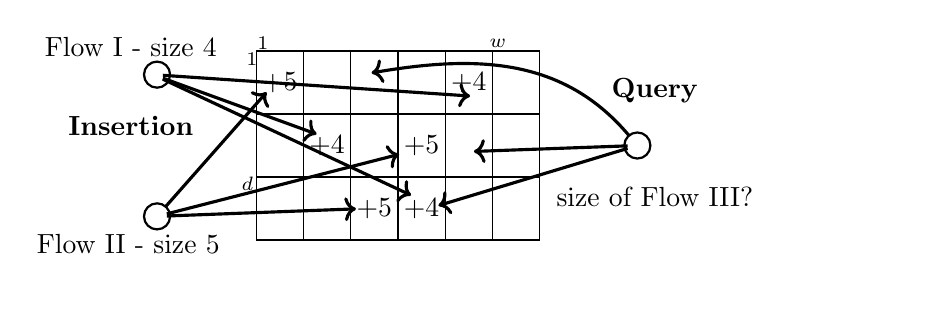
\begin{tikzpicture}
 \foreach \c/\i [count=\n] in  
        {white/4,white/0, white/0,white/0,white/9,white/0} 
           \node[draw,fill=\c,minimum height=0.8cm,minimum width = 0.6cm,xshift=(\n+2.1)*0.6cm](B\n){};
            \foreach \c/\i [count=\n] in  
        {white/4,white/0, white/0,white/0,white/9,white/0} 
           \node[draw,fill=\c,minimum height=0.8cm,minimum width = 0.6cm,xshift=(\n+2.1)*0.6cm, yshift =0.8cm](B\n){} ;
            \foreach \c/\i [count=\n] in 
        {white/4,white/0, white/0,white/0,white/9,white/0} 
           \node[draw,fill=\c,minimum height=0.8cm,minimum width = 0.6cm,xshift=(\n+2.1)*0.6cm, yshift =1.6cm](B\n){} ;
         \foreach \j [count=\m] in  
        {0,1,2,3,4,5,6,7,8,9,10,11,12,13,14} 
           \node[] (q\m) at (\m*0.5cm,0.36) {}; 
\node[text width=0.75cm, anchor=west, right] at (0.73,-1.0) {};
\node[text width=0.75cm, anchor=west, right] at (2.31,-1.0) {};
 \foreach \j [count=\m] in  
        {1,1,2,3,4,5,6,7,8,9,10,11,12} 
           \node[] (z\m) at (\m*0.5cm,-0.46) {}; 
\node[text width=3.5cm, anchor=west, right] at (-1.25,2.05) {Flow I - size 4};
\node[draw,circle,scale=1.0, thick] at (0.30,1.7) {}; 
\node [] (n0) at (0.25,1.7) {};
\node [] (z1) at (4.40,1.42) {};
\node [] (z2) at (2.45,0.9) {};
\node [] (z3) at (3.65,0.11) {};
\draw[line width=0.04cm, ->] (n0) -- (z1);
\draw[line width=0.04cm, ->] (n0) -- (z2);
\draw[line width=0.04cm, ->] (n0) -- (z3);

\node[text width=0.5cm, anchor=west, right] at (2.11,0.8) {$+4$};
\node[text width=0.5cm, anchor=west, right] at (3.91,1.6) {$+4$};
\node[text width=0.5cm, anchor=west, right] at (3.31,0.0) {$+4$};
\node[text width=0.5cm, anchor=west, right] at (2.71,0.0) {$+5$};
\node[text width=0.5cm, anchor=west, right] at (3.31,0.8) {$+5$};
\node[text width=0.5cm, anchor=west, right] at (1.51,1.6) {$+5$};
%\draw[->] (n0) -- (-0.4,+0.46);
%\draw[->] (n0) -- (q3);

\node[text width=0.5cm, anchor=west, right] at (1.45,2.10) {\scriptsize $1$};
\node[text width=0.5cm, anchor=west, right] at (4.40,2.10) {\scriptsize $w$};

\node[text width=0.5cm, anchor=west, right] at (1.31,1.90) {\scriptsize $1$};
\node[text width=0.5cm, anchor=west, right] at (1.25,0.32) {\scriptsize $d$};


\node[draw,circle,scale=1.0, thick] at (0.30,-0.1) {};
\node[text width=3.5cm, anchor=west, right] at (-1.35,-0.45) {Flow II - size 5};
\node [] (nl) at (0.30,-0.1) {};
\node [] (nl1) at (1.80,1.6) {};
\node [] (nl2) at (3.5,0.72) {};
\node [] (nl3) at (2.95,0.0) {};
\draw[line width=0.04cm, ->] (nl) -- (nl1);
\draw[ line width=0.04cm, ->] (nl) -- (nl2);
\draw[line width=0.04cm, ->] (nl) -- (nl3);


\node[draw,circle,scale=1.0, thick] at (6.40,0.8) {};
\node[text width=3.5cm, anchor=west, right] at (5.25,0.15) {size of Flow III?};
\node [] (n2) at (6.4,0.8) {};

\node [] (n21) at (2.90,1.7) {};
\node [] (n22) at (4.2,0.72) {}; 
\node [] (n23) at (3.75,0.0) {};
%\draw[blue, line width=0.04cm, ->] (n2) --  (n21);
\draw [->, line width=0.04cm] (n2) to [out=130,in=10] (n21);
\draw[line width=0.04cm, ->] (n2) -- (n22);
%\draw [->, line width=0.04cm] (n2) to [out=200,in=290] (n23);
\draw[line width=0.04cm, ->] (n2) -- (n23);
\node[text width=3.5cm, anchor=west, right] at (-0.95,1.05) {\textbf{Insertion}};
\node[text width=3.5cm, anchor=west, right] at (5.95,1.5) {\textbf{Query}};
%\draw[->] (nl) -- (q3);
%\draw[->] (nl) -- (q8);
%\node[text width=3.5cm, anchor=west, right] at (4.60,1.75) {Flow III - size 1};
%\node[draw,circle,scale=1.0, thick] at (5.29,1.4) {};
%\node [] (n2) at (5.3,1.3) {};
%\draw[->] (n2) -- (q8); 
%\draw[->] (n2) -- (q11); 
%\node[draw,circle,scale=1.0, thick] at (2.59,-1.4) {};
%\node[text width=4.0cm, anchor=west, right] at (1.51,-1.7) {size of Flow II?};
%\node [] (n3) at (2.6,-1.3) {};
%\draw[->] (n3) -- (z3);
%\draw[->] (n3) -- (z8);
\end{tikzpicture}
\caption{\label{sktc-fig:CM} The Count-Min sketch (CM)~\cite{CountMin}, allowing flow size estimation. \inred{Each flow is mapped to a single counter in each row. Flow I is mapped to counter 5 in row 1, counter 2 in row 2, and counter 4 in row 3. The mappings are presented in the figure.} A flow size is estimated as the minimum among the counters it is mapped to by a set of hash functions.}	
\end{figure}

The CM  is illustrated in Figure~\ref{sktc-fig:CM}. Flows I, II  of size 4, and 5, respectively, are recorded in the sketch (shown on the left side). Each flow increases the value of $d=3$ counters by its size.  The size of Flow III (right side) is estimated by querying the CM  as the minimal among the $d$ counters it is mapped to.

%As for every sketch, the estimation generated from the Count-Min sketch is imperfect and can be overestimated.
\inred{While, as mentioned, the CM can observe overestimations~\cite{CountMin}}, the accuracy guarantees can be described as follows:
When using CM with width $w$ and depth $d$ the estimation $\hat{f}$ of flow $f$ satisfies with probability $1-\delta$
\[\hat{f} \leq f + \epsilon N.\]
Here, $N$ is the number of packets in the measured stream, $\epsilon$ holds $w = \left\lceil \frac{e}{\epsilon} \right\rceil$ (for Euler's number $e$) and $\delta$ holds $d= \left\lceil \ln\frac{1}{\delta} \right\rceil$.

\subsubsection{KMV (\emph{K-minimum-values}) Sketch}  \label{sktc-ssec:kmv}

Another essential capability in network monitoring is the ability to estimate the number of distinct flows, called stream cardinality. Counting the exact stream cardinality is generally challenging in high traffic rate, making it hard to save some unique data for each flow and quickly identify whether a flow has previously appeared or not. 

The $K$-minimum-values sketch (KMV)~\cite{giroire2009order, KMV} uses a hash function $h$ that maps every flow uniformly to $[0,1]$. For a parameter $k$, the sketch maintains the minimal $k$ observed values for flows so far. Let $h_1,...,h_k$ be those $k$ minimal calculated values such that $h_1<h_2<...<h_k$. The \emph{KMV} sketch provides its cardinality estimation as $\frac{k}{h_k}$. This estimation is based on the fact that the $k$ order statistics of group uniformly randomized in the range $[0,1]$ is equal to $\frac{k}{n+1}$. The error of the algorithm is $\frac{1}{\sqrt{k}}$, i.e.  for $m$ flows, the KMV sketch estimation $m'$ satisfies $\left|\frac{m-m'}{m}\right| = O(\frac{1}{\sqrt{k}})$.

\begin{figure}[!t]%[!ht]
	\centering
	

\tikzset{every picture/.style={line width=0.75pt}} %set default line width to 0.75pt        

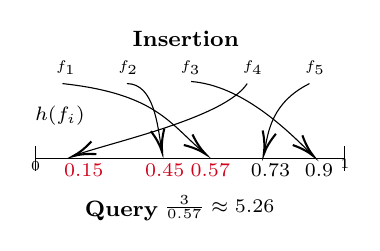
\begin{tikzpicture}[x=0.75pt,y=0.75pt,yscale=-1,xscale=1]
%uncomment if require: \path (0,300); %set diagram left start at 0, and has height of 300

%Straight Lines [id:da2080794547555267] 
\draw    (101.5,100.67) -- (250.5,100.67) ;
%Straight Lines [id:da6803929792177787] 
\draw    (101.5,94.67) -- (101.5,106.67) ;
%Straight Lines [id:da0782789730692306] 
\draw    (250.5,94.67) -- (250.5,106.67) ;
%Curve Lines [id:da9195899812176473] 
\draw    (114.5,64.67) .. controls (159.12,69.52) and (166.1,83.78) .. (182,97.4) ;
\draw [shift={(183.5,98.67)}, rotate = 219.47] [color={rgb, 255:red, 0; green, 0; blue, 0 }  ][line width=0.75]    (10.93,-3.29) .. controls (6.95,-1.4) and (3.31,-0.3) .. (0,0) .. controls (3.31,0.3) and (6.95,1.4) .. (10.93,3.29)   ;
%Curve Lines [id:da2342594252069674] 
\draw    (145.5,64.67) .. controls (158.66,64.67) and (160.33,84.99) .. (162.15,95.73) ;
\draw [shift={(162.5,97.67)}, rotate = 258.69] [color={rgb, 255:red, 0; green, 0; blue, 0 }  ][line width=0.75]    (10.93,-3.29) .. controls (6.95,-1.4) and (3.31,-0.3) .. (0,0) .. controls (3.31,0.3) and (6.95,1.4) .. (10.93,3.29)   ;
%Curve Lines [id:da7520327389763415] 
\draw    (176.5,63.67) .. controls (200.63,65.6) and (221.96,86.15) .. (234.2,98.37) ;
\draw [shift={(235.5,99.67)}, rotate = 225] [color={rgb, 255:red, 0; green, 0; blue, 0 }  ][line width=0.75]    (10.93,-3.29) .. controls (6.95,-1.4) and (3.31,-0.3) .. (0,0) .. controls (3.31,0.3) and (6.95,1.4) .. (10.93,3.29)   ;
%Curve Lines [id:da8707723296036518] 
\draw    (203.5,64.67) .. controls (192.89,81.07) and (138.5,92.82) .. (121.23,99.01) ;
\draw [shift={(119.5,99.67)}, rotate = 338.2] [color={rgb, 255:red, 0; green, 0; blue, 0 }  ][line width=0.75]    (10.93,-3.29) .. controls (6.95,-1.4) and (3.31,-0.3) .. (0,0) .. controls (3.31,0.3) and (6.95,1.4) .. (10.93,3.29)   ;
%Curve Lines [id:da46923256267070834] 
\draw    (233.5,64.67) .. controls (215,73.92) and (213.61,88.3) .. (211.93,96.74) ;
\draw [shift={(211.5,98.67)}, rotate = 284.04] [color={rgb, 255:red, 0; green, 0; blue, 0 }  ][line width=0.75]    (10.93,-3.29) .. controls (6.95,-1.4) and (3.31,-0.3) .. (0,0) .. controls (3.31,0.3) and (6.95,1.4) .. (10.93,3.29)   ;

% Text Node
\draw (98,101) node [anchor=north west][inner sep=0.75pt]   [align=left] {{\tiny 0}};
% Text Node
\draw (247,100) node [anchor=north west][inner sep=0.75pt]   [align=left] {{\tiny 1}};
% Text Node
\draw (110,52.4) node [anchor=north west][inner sep=0.75pt]  [font=\tiny]  {${\displaystyle f_{1}}$};
% Text Node
\draw (140,52.4) node [anchor=north west][inner sep=0.75pt]  [font=\tiny]  {${\displaystyle f_{2}}$};
% Text Node
\draw (170,52.4) node [anchor=north west][inner sep=0.75pt]  [font=\tiny]  {${\displaystyle f_{3}}$};
% Text Node
\draw (200,52.4) node [anchor=north west][inner sep=0.75pt]  [font=\tiny]  {${\displaystyle f_{4}}$};
% Text Node
\draw (230,52.4) node [anchor=north west][inner sep=0.75pt]  [font=\tiny]  {${\displaystyle f_{5}}$};
% Text Node
\draw (147,38) node [anchor=north west][inner sep=0.75pt]   [align=left] {\textbf{{\footnotesize Insertion}}};
% Text Node
\draw (230,102) node [anchor=north west][inner sep=0.75pt]   [align=left] {{\scriptsize 0.9}};
% Text Node
\draw (204,102) node [anchor=north west][inner sep=0.75pt]   [align=left] {{\scriptsize 0.73}};
% Text Node
\draw (175,102) node [anchor=north west][inner sep=0.75pt]  [color={rgb, 255:red, 208; green, 2; blue, 27 }  ,opacity=1 ] [align=left] {{\scriptsize 0.57}};
% Text Node
\draw (114,102) node [anchor=north west][inner sep=0.75pt]  [color={rgb, 255:red, 208; green, 2; blue, 27 }  ,opacity=1 ] [align=left] {{\scriptsize 0.15}};
% Text Node
\draw (153,102) node [anchor=north west][inner sep=0.75pt]  [color={rgb, 255:red, 208; green, 2; blue, 27 }  ,opacity=1 ] [align=left] {{\scriptsize 0.45}};
% Text Node
\draw (100,74.4) node [anchor=north west][inner sep=0.75pt]  [font=\scriptsize]  {$h( f_{i})$};
% Text Node
\draw (124,120) node [anchor=north west][inner sep=0.75pt]   [align=left] {\textbf{{\footnotesize Query}}};
% Text Node
\draw (162,117.4) node [anchor=north west][inner sep=0.75pt]  [font=\scriptsize]  {$\frac{3}{0.57} \approx 5.26$};


\end{tikzpicture}

    \caption{The $K$-minimum-values sketch (KMV) \cite{giroire2009order, KMV}, allowing cardinality estimation. The cardinality is estimated by dividing $k$ with the $k$'th minimal hashed value, (here $k=3$ with recorded values shown in red).}
    \label{sktc-fig:kmv-example}
\end{figure}

The KMV is illustrated in Figure \ref{sktc-fig:kmv-example}. There are five flows recorded in the sketch, each maps to a different value in the range of $[0,1]$. Here $k=3$ so that only the three minimal values are stored. When flows' cardinality is queried, the sketch finds the largest value that is currently stored, which is $0.57$ and returns $\frac{k}{0.57} = \frac{3}{0.57} \approx 5.26$ distinct flows.

\subsubsection{HyperLogLog for Cardinality Estimation}
\label{sktc-ssec:HyperLogLog}

% \begin{algorithm}[!h]
% \DontPrintSemicolon
% \KwIn{
% Stream of elements $A = (a_1, \ldots, a_k)$.
% }
% \KwOut{
% Estimated number of distinct elements in $A$
% }
% $M[0] = \ldots = M[m-1] = 0$, $d= \log_2(m)$, $\alpha_m  = 0.7213 / (1+1.079/m)$ for $m \ge 128$;

% \For{$a_i \in A$} {
% $(b_1, \ldots, b_d, b_{d+1}, \ldots, b_{d+t}) = h(a_i)$ \\
% $j =  (b_1, \ldots, b_d)$\\
% $M[j] = \max(M[j], \rho((b_{d+1}, \ldots, b_{d+t})))$
% }
% $Z = \Big(\sum_{j = 0}^{m-1} {2^{-M[j]}}\Big)^{-1}$\\
% \Return $\alpha_m  \cdot m^2 \cdot Z$\\
% \caption{The \emph{HyperLogLog} algorithm for cardinality estimation~\cite{HyperLogLog}}
% %for estimating number of distinct elements
% \label{sktc-Alg_HyperLogLog}
% \end{algorithm}



HyperLogLog (HLL)~\cite{Flajolet07hyperloglog,heule2013hyperloglog} is another popular algorithm for cardinality estimation.
As a building block, it relies on the Flajolet–Martin method of estimating the number of distinct elements~\cite{flajolet1983probabilistic, LogLog}. They propose computing a hash value $h(a_i)$ for each element $a_i$ and a value $\rho(h(a_i))$ that indicates the index of the first non-zero bit upon considering the binary representation of $h(a_i)$, starting from the least significant bit. 
The HLL holds an array $M$ of $m=2^d$ counters. For an element $a_i$, a counter is selected based on the $d$ left-most bits in $h(a_i)$ and this counter is potentially updated based on the next $t$ bits in  $h(a_i)$. 
The use of hashing ensures that repeated elements in the stream imply the same values and thus cannot increase the counter values. Finally, \inblue{the cardinality estimation} computed based on the $m$ counters is:
\[\alpha_m  \cdot m^2 \cdot \big(\sum_{j = 0}^{m-1} {2^{-M[j]}}\big)^{-1}.\]
$\alpha_m$ is approximated as:
\[\alpha_m=\begin{cases}
0.673 & m=16 \\
0.697 & m=32 \\
0.706 & m=64 \\
\frac{0.723}{1+\frac{1.079}{m}} & m \geq 128
\end{cases}\]
as shown in~\cite{Flajolet07hyperloglog}.
% The pseudocode for the HLL algorithm is shown in Algorithm ~\ref{sktc-Alg_HyperLogLog}. 

\subsubsection{Maximum Merging (MM)} \label{sktc-ssec:mm}

\inblue{
Previous work by Yang et al. has presented the Maximum Merging (\textbf{MM})~\cite{yang2018elastic} method, a method for compressing CM before transmission over the network. In this method, the CM sketch is compressed from size $w$ to $w'$, where $w'$ is a divisor of $w$. Column $i$ is added to column $(i \mod w')$. If $w = r \cdot w'$, the CM sketch is compressed by} \ingreen{a factor}  \inblue{$r$ earlier to its transmission over the network.
}

\forRevThree{
While this method maintains the lookup speed of the original CM sketch, a limitation of this method is the requirement that $w'$ be a divisor of $w$.
%}
%\forRevThree{ 
Even more important, in the common  scenario of multiple measurements,  
the MM scheme compresses all sketches equally regardless of the amount of traffic each of them observes. 
We indicate that this scheme can lead to under utilized bandwidth. For example, if the two node processed different portions of the stream, an identical compression implies over-compression of the sketch that observes more traffic, leading to a higher overall error.} %We explain that typically the sketch that observed a smaller portion of the traffic can be further compressed without affecting much the overall error. }

%Furthermore, if the traffic distribution was not equal, i.e., one node processed a much larger portion of the stream, the MM scheme applies equal compression to both nodes. For example, consider the case where node 1 processes $90\%$ of the stream and node 2 processes $10\%$ of it. Under MM compression, both nodes send a similar summary size.

%We propose having node 2 highly compress its summary, and node 1 compressing it less than in MM. While in this case node 1 sends a larger summary than in MM, the sum of the compressed sizes in MM is greater than the sum of our proposed compressed sizes, while the error remains similar. I.e., we use less bandwidth while achieving a similar error.

\subsection{Related Work} \label{sktc-ssec:related-work}

Common sketch solutions focus on the trade-off of speed, accuracy, and memory (e.g.,~\cite{CountMin, cormode2011sketch, metwally2005efficient, sivaraman2017heavy, estan2003new,  9667240, 9068483, Rottenstreich21} and more). However, they generally consider only a single node ingesting the entire stream.
The introduction of software-defined networks (SDN) allows for deploying
centralized algorithms for maintaining and collecting information about network
operations~\cite{yu2013software}. These solutions typically have a centralized controlled merging
of incoming data from ingestion nodes. Network-wide measurements have
been widely studied~\cite{afek2018detecting,anderson2017high,li2016flowradar,harrison2020carpe}. These solutions, however, do not consider the size of control packets sent to the controller -- they do not take into account that these control packets may worsen existing congestion~\cite{zhang2010optimizing, benson2010understanding}.

 Shrivastava et al.\cite{shrivastava2016time} presented time adaptive sketches and discussed the need for having recent data more accessible. In \cite{harrison2018network}, Harrison et al. presented a network-wide scheme of detecting heavy-hitters while considering the reporting communication overhead. \cite{harrison2020carpe} presented a method of heavy-hitters detection that used probabilistic summary reporting to decrease control packets during DDoS attacks. These two works emphasize that minimizing summaries size is critical and can have a major influence on network performance. By using methods of our paper, network operators can create larger sketches and excess the need for time-reliant sketches. 


Recently,~\cite{FPFZCM} suggested methods for accurate flow size estimation in the Count-Min sketch (CM)  without overestimation, that apply when the number of flows of non-zero size is bounded. 
Yang et al. presented the Maximum Merging (\textbf{MM})~\cite{yang2018elastic}, a method for compressing CM before transmission over the network. MM allows providing estimations under a range of traffic characteristics implying various bandwidth constraints. The main limitation of this method is that it can only compress the CM to a constant $w'$ which divides the width $w$.
\forRevThree{
MM does not deal with two aspects that we find important for making it practical. It refers to a single sketch and does not discuss the compression of multiple sketch instances and in particular how to compute various compression ratios for such sketches based on the traffic. Likewise, it is focused solely on the CM. In this work, we study the common scenario of multiple distributed sketches and refer in addition to CM also to other common sketches. 
}


\forRevThree{
Our methods utilize similar patterns to the original sketches, therefore our proposed sketches and techniques may have the potential to be implemented on programmable switches. 
For example, the following sketches have been implemented using the Tofino architecture~\cite{tofino}:
the CM sketch~\cite{namkung2021telemetry}, the Quantiles sketch~\cite{ivkin2019qpipe}, and more~\cite{zhang2021cocosketch, hang2019interleaved, zeno2020swishmem}.}

%\forRevThree{As mentioned, the Elastic Sketch~\cite{yang2018elastic} presented a compression method for sketches, to adapt to available network bandwidth using the MM technique, detailed in Section~\ref{sktc-ssec:mm}. MM allows providing estimations under a range of traffic characteristics implying various bandwidth constraints. It refers to a single instance of the CM Elastic Sketch However, unlike our SKTC compression approach,  and does not discuss how to use multiple instances of the Elastic Sketch for a single distributed sketch. We refer to the MM technique as a baseline scheme in the evaluations.}


%UnivMon~\cite{liu2016one} and NitroSketch~\cite{NitroSketch} summarize streams in a sketch that can later answer multiple measurement tasks. The SKTC compression approach can be generalized to such sketches, while the analysis of the ideal resize factors can be generalized to refer jointly to the accuracy of multiple tasks. \inblue{To the best of our knowledge, only the Elastic Sketch adapts to \inred{available network bandwidth}~\cite{yang2018elastic} using the MM technique. It is proposed to continuously provide estimations under all traffic characteristics, \inred{i.e., provide estimations under all network scenarios, e.g., in low-bandwidth conditions when the network is undergoing a DDoS attack. They do not discuss how to use multiple instances of the Elastic Sketch for a single distributed sketch. Our main point of comparison with the Elastic Sketch is the MM compression technique.}}

\section{The CM-SKTC Compression Method}\label{sktc-sec:com-sketch}
We present a method that allows compressing any sized CM ($d,w$) to any new size possible ($d,w'$) for $w' \in [1,w]$. 
Let $h_1, \dots ,h_d$ be \inblue{pair-wise independent} hash functions used in original CM, such that every function holds $h_i : \{f_1,f_2, \dots\} \mapsto \{1,2, \dots, w\}$, \inblue{where $f_j$ is flow $j$}. Let $g_1,...,g_d$ be \inblue{pair-wise independent} hash functions such that $g_i : \{1,2, \dots, w\} \mapsto \{1,2, \dots, w'\}$ for every $i$. 

The CM-SKTC compression method works as follows. For each array $\textsl{S}^c[j]$ in the sketch, the value of the $l$'s cell $\textsl{S}^c[j][l]$ is the maximum value over all cells in the corresponding array of the original sketch $\textsl{S}[j]$ that by the hash function $g_j$ are hashed to the $l$'th cell (i.e. $\textsl{S}^c[j][l] \gets \max\limits_{i: g_j(i) = l} \{ \textsl{S}[j][i]\}$). Algorithm~\ref{sktc-alg:w-compression} presents the CM-SKTC compression method pseudo code.

An example of the compression process of CM-SKTC is illustrated in Figure \ref{sktc-fig:cm-sktc-example} where a CM-SKTC of size  $d=2, w'=4$ is computed for a CM of size $d=2, w=6$. Notice that the method reduces the number of columns (rather than that of the rows) since typically the number of rows is low beforehand, as there is a need for a distinct hash function per row.

The query method (Algorithm \ref{sktc-alg:w-compression-query}) from CM-SKTC is similar to the original CM query. When flow $f$ estimation value is required, for each array $\textsl{S}^c[j]$ (where $j \in [1,d]$) find the appropriate cell  $\textsl{S}^c[j][g_j\left(h_j(f)\right)]$ (one in each array) and return their respective minimal value. 

%One can see that as Zip sketch cannot create an under-estimated result,  
Similar to the original CM and the \textbf{MM}~\cite{yang2018elastic},  the CM-SKTC method also generates only overestimation values. 

% Change the algorithm to be O(wd) instead of O(w'dw)
\setlength{\textfloatsep}{2pt}
\begin{algorithm}[t!]
\begin{algorithmic}[1]
		\REQUIRE{A CM \textsl{S}  (size $d \times w$), new width $w'$}
		\ENSURE{Compressed CM-SKTC \textsl{S}$^c$ with size $d \times w'$}
		
		\STATE $\textsl{S}^c \gets $ array of $0$'s of size $d \times w'$
		\FOR{$j=1; \ j\leq d;\ j++$}
            \FOR{$i=1; \ i\leq w;\ i++$}
                \STATE $l=g_j(i)$
                \STATE  $S^c[j][l] = \max(S^c[j][l], S[j][i])$ 
   %             \IF{$S[j][i] > S^c[j][l]$}
%                    \STATE $S^c[j][l] = S[j][i]$
%                \ENDIF
            \ENDFOR
        \ENDFOR
		\RETURN $\textsl{S}^c$
	\end{algorithmic}
	\caption{CM-SKTC compression algorithm}
	\label{sktc-alg:w-compression}
\end{algorithm}

\begin{figure}[t!]
    \centering
    

\tikzset{every picture/.style={line width=0.75pt}} %set default line width to 0.75pt        

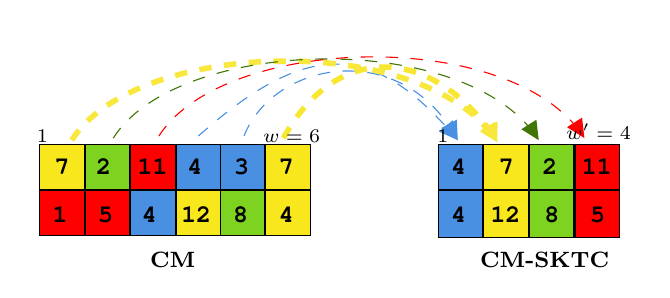
\begin{tikzpicture}[x=0.75pt,y=0.75pt,yscale=-1,xscale=1]
%uncomment if require: \path (0,300); %set diagram left start at 0, and has height of 300

%Shape: Rectangle [id:dp9120519996767289] 
\draw  [fill={rgb, 255:red, 248; green, 231; blue, 28 }  ,fill opacity=1 ] (39,134) -- (60.5,134) -- (60.5,156) -- (39,156) -- cycle ;
%Shape: Rectangle [id:dp5578762422129069] 
\draw  [fill={rgb, 255:red, 126; green, 211; blue, 33 }  ,fill opacity=1 ] (61,134) -- (82.5,134) -- (82.5,156) -- (61,156) -- cycle ;
%Shape: Rectangle [id:dp5149322189764962] 
\draw  [fill={rgb, 255:red, 255; green, 0; blue, 0 }  ,fill opacity=1 ] (83,134) -- (104.5,134) -- (104.5,156) -- (83,156) -- cycle ;
%Shape: Rectangle [id:dp8371364169912505] 
\draw  [fill={rgb, 255:red, 74; green, 144; blue, 226 }  ,fill opacity=1 ] (105,134) -- (126.5,134) -- (126.5,156) -- (105,156) -- cycle ;
%Shape: Rectangle [id:dp8774137890100953] 
\draw  [fill={rgb, 255:red, 74; green, 144; blue, 226 }  ,fill opacity=1 ] (126,134) -- (147.5,134) -- (147.5,156) -- (126,156) -- cycle ;
%Shape: Rectangle [id:dp8260064759507215] 
\draw  [fill={rgb, 255:red, 248; green, 231; blue, 28 }  ,fill opacity=1 ] (148,134) -- (169.5,134) -- (169.5,156) -- (148,156) -- cycle ;
%Shape: Rectangle [id:dp13750697143490287] 
\draw  [fill={rgb, 255:red, 255; green, 0; blue, 0 }  ,fill opacity=1 ] (39,156) -- (60.5,156) -- (60.5,178) -- (39,178) -- cycle ;
%Shape: Rectangle [id:dp12750267479029076] 
\draw  [fill={rgb, 255:red, 255; green, 0; blue, 0 }  ,fill opacity=1 ] (61,156) -- (82.5,156) -- (82.5,178) -- (61,178) -- cycle ;
%Shape: Rectangle [id:dp9453531436538745] 
\draw  [fill={rgb, 255:red, 74; green, 144; blue, 226 }  ,fill opacity=1 ] (83,156) -- (104.5,156) -- (104.5,178) -- (83,178) -- cycle ;
%Shape: Rectangle [id:dp019183616299335293] 
\draw  [fill={rgb, 255:red, 248; green, 231; blue, 28 }  ,fill opacity=1 ] (105,156) -- (126.5,156) -- (126.5,178) -- (105,178) -- cycle ;
%Shape: Rectangle [id:dp9174572360745898] 
\draw  [fill={rgb, 255:red, 126; green, 211; blue, 33 }  ,fill opacity=1 ] (126,156) -- (147.5,156) -- (147.5,178) -- (126,178) -- cycle ;
%Shape: Rectangle [id:dp2814590512908379] 
\draw  [fill={rgb, 255:red, 248; green, 231; blue, 28 }  ,fill opacity=1 ] (148,156) -- (169.5,156) -- (169.5,178) -- (148,178) -- cycle ;
%Shape: Rectangle [id:dp3867673825425666] 
\draw  [fill={rgb, 255:red, 74; green, 144; blue, 226 }  ,fill opacity=1 ] (231,134) -- (252.5,134) -- (252.5,157) -- (231,157) -- cycle ;
%Shape: Rectangle [id:dp45900611803416114] 
\draw  [fill={rgb, 255:red, 248; green, 231; blue, 28 }  ,fill opacity=1 ] (253,134) -- (274.5,134) -- (274.5,157) -- (253,157) -- cycle ;
%Shape: Rectangle [id:dp14536752724329527] 
\draw  [fill={rgb, 255:red, 126; green, 211; blue, 33 }  ,fill opacity=1 ] (275,134) -- (296.5,134) -- (296.5,157) -- (275,157) -- cycle ;
%Shape: Rectangle [id:dp7559601744598143] 
\draw  [fill={rgb, 255:red, 255; green, 0; blue, 0 }  ,fill opacity=1 ] (297,134) -- (318.5,134) -- (318.5,157) -- (297,157) -- cycle ;
%Shape: Rectangle [id:dp5499444494363386] 
\draw  [fill={rgb, 255:red, 74; green, 144; blue, 226 }  ,fill opacity=1 ] (231,156) -- (252.5,156) -- (252.5,179) -- (231,179) -- cycle ;
%Shape: Rectangle [id:dp6548836133040838] 
\draw  [fill={rgb, 255:red, 248; green, 231; blue, 28 }  ,fill opacity=1 ] (253,156) -- (274.5,156) -- (274.5,179) -- (253,179) -- cycle ;
%Shape: Rectangle [id:dp5995721454141998] 
\draw  [fill={rgb, 255:red, 126; green, 211; blue, 33 }  ,fill opacity=1 ] (275,156) -- (296.5,156) -- (296.5,179) -- (275,179) -- cycle ;
%Shape: Rectangle [id:dp8157813465457489] 
\draw  [fill={rgb, 255:red, 255; green, 0; blue, 0 }  ,fill opacity=1 ] (297,156) -- (318.5,156) -- (318.5,179) -- (297,179) -- cycle ;
%Curve Lines [id:da7793812944008702] 
\draw [color={rgb, 255:red, 74; green, 144; blue, 226 }  ,draw opacity=1 ] [dash pattern={on 4.5pt off 4.5pt}]  (115.5,130) .. controls (166.72,84.69) and (198.54,83.04) .. (238.66,129.83) ;
\draw [shift={(240.5,132)}, rotate = 230.07999999999998] [fill={rgb, 255:red, 74; green, 144; blue, 226 }  ,fill opacity=1 ][line width=0.08]  [draw opacity=0] (8.93,-4.29) -- (0,0) -- (8.93,4.29) -- cycle    ;
%Curve Lines [id:da17576300112648635] 
\draw [color={rgb, 255:red, 74; green, 144; blue, 226 }  ,draw opacity=1 ] [dash pattern={on 4.5pt off 4.5pt}]  (137.5,130) .. controls (151.29,94.54) and (211.65,82.37) .. (239.26,129.79) ;
\draw [shift={(240.5,132)}, rotate = 241.63] [fill={rgb, 255:red, 74; green, 144; blue, 226 }  ,fill opacity=1 ][line width=0.08]  [draw opacity=0] (8.93,-4.29) -- (0,0) -- (8.93,4.29) -- cycle    ;
%Curve Lines [id:da12939079412155663] 
\draw [color={rgb, 255:red, 248; green, 231; blue, 50 }  ,draw opacity=2 ] [dash pattern={on 4.5pt off 4.5pt}][line width=2]  (156.5,131) .. controls (181.25,85.65) and (226.58,85.07) .. (258.54,130.92) ;
\draw [shift={(259.5,133)}, rotate = 245.43] [fill={rgb, 255:red, 248; green, 231; blue, 60 }  ,fill opacity=1 ][line width=0.5]  [draw opacity=0] (8.93,-4.29) -- (0,0) -- (8.93,4.29) -- cycle    ;
%Curve Lines [id:da23437502293589474] 
\draw [color={rgb, 255:red, 248; green, 231; blue, 60 }  ,draw opacity=1, line width=0.5 ] [dash pattern={on 4.5pt off 4.5pt}][line width=2]  (54.5,132) .. controls (85.04,83.73) and (221.32,79.13) .. (257.9,130.61) ;
\draw [shift={(259.5,133)}, rotate = 237.8] [fill={rgb, 255:red, 248; green, 231; blue, 60 }  ,fill opacity=1 ][line width=0.5]  [draw opacity=0] (8.93,-4.29) -- (0,0) -- (8.93,4.29) -- cycle    ;
%Curve Lines [id:da16470429934928688] 
\draw [color={rgb, 255:red, 65; green, 117; blue, 5 }  ,draw opacity=1 ] [dash pattern={on 4.5pt off 4.5pt}]  (74.5,131) .. controls (105.04,82.73) and (241.32,78.13) .. (277.9,129.61) ;
\draw [shift={(279.5,132)}, rotate = 237.8] [fill={rgb, 255:red, 65; green, 117; blue, 5 }  ,fill opacity=1 ][line width=0.08]  [draw opacity=0] (8.93,-4.29) -- (0,0) -- (8.93,4.29) -- cycle    ;
%Curve Lines [id:da3875594417212562] 
\draw [color={rgb, 255:red, 255; green, 0; blue, 0 }  ,draw opacity=1 ] [dash pattern={on 4.5pt off 4.5pt}]  (96.5,130) .. controls (124.04,86.47) and (237.6,78.45) .. (286.45,115.07) .. controls (291.73,119.02) and (296.25,123.5) .. (299.83,128.51) ;
\draw [shift={(301.5,131)}, rotate = 237.8] [fill={rgb, 255:red, 255; green, 0; blue, 0 }  ,fill opacity=1 ][line width=0.08]  [draw opacity=0] (8.93,-4.29) -- (0,0) -- (8.93,4.29) -- cycle    ;

% Text Node
\draw (44,163) node [anchor=north west][inner sep=0.75pt]  [font=\large,color={rgb, 255:red, 0; green, 0; blue, 0 }  ,opacity=1 ] [align=left] {{\fontfamily{pcr}\selectfont \textbf{{\small 1}}}};
% Text Node
\draw (66,163) node [anchor=north west][inner sep=0.75pt]  [font=\large,color={rgb, 255:red, 0; green, 0; blue, 0 }  ,opacity=1 ] [align=left] {{\fontfamily{pcr}\selectfont {\small \textbf{5}}}};
% Text Node
\draw (87,163) node [anchor=north west][inner sep=0.75pt]  [font=\large,color={rgb, 255:red, 0; green, 0; blue, 0 }  ,opacity=1 ] [align=left] {{\fontfamily{pcr}\selectfont {\small \textbf{4}}}};
% Text Node
\draw (106,163) node [anchor=north west][inner sep=0.75pt]  [font=\large,color={rgb, 255:red, 0; green, 0; blue, 0 }  ,opacity=1 ] [align=left] {{\fontfamily{pcr}\selectfont {\small \textbf{12}}}};
% Text Node
\draw (131,163) node [anchor=north west][inner sep=0.75pt]  [font=\large,color={rgb, 255:red, 0; green, 0; blue, 0 }  ,opacity=1 ] [align=left] {{\fontfamily{pcr}\selectfont {\small \textbf{8}}}};
% Text Node
\draw (153,163) node [anchor=north west][inner sep=0.75pt]  [font=\large,color={rgb, 255:red, 0; green, 0; blue, 0 }  ,opacity=1 ] [align=left] {{\fontfamily{pcr}\selectfont {\small \textbf{4}}}};
% Text Node
\draw (236,163) node [anchor=north west][inner sep=0.75pt]  [font=\large,color={rgb, 255:red, 0; green, 0; blue, 0 }  ,opacity=1 ] [align=left] {{\fontfamily{pcr}\selectfont {\small \textbf{4}}}};
% Text Node
\draw (255,163) node [anchor=north west][inner sep=0.75pt]  [font=\large,color={rgb, 255:red, 0; green, 0; blue, 0 }  ,opacity=1 ] [align=left] {{\fontfamily{pcr}\selectfont {\small \textbf{12}}}};
% Text Node
\draw (281,163) node [anchor=north west][inner sep=0.75pt]  [font=\large,color={rgb, 255:red, 0; green, 0; blue, 0 }  ,opacity=1 ] [align=left] {{\fontfamily{pcr}\selectfont {\small \textbf{8}}}};
% Text Node
\draw (303,163) node [anchor=north west][inner sep=0.75pt]  [font=\large,color={rgb, 255:red, 0; green, 0; blue, 0 }  ,opacity=1 ] [align=left] {{\fontfamily{pcr}\selectfont {\small \textbf{5}}}};
% Text Node
\draw (45,140) node [anchor=north west][inner sep=0.75pt]  [font=\large,color={rgb, 255:red, 0; green, 0; blue, 0 }  ,opacity=1 ] [align=left] {{\fontfamily{pcr}\selectfont \textbf{{\small 7}}}};
% Text Node
\draw (153,140) node [anchor=north west][inner sep=0.75pt]  [font=\large,color={rgb, 255:red, 0; green, 0; blue, 0 }  ,opacity=1 ] [align=left] {{\fontfamily{pcr}\selectfont \textbf{{\small 7}}}};
% Text Node
\draw (65,140) node [anchor=north west][inner sep=0.75pt]  [font=\large,color={rgb, 255:red, 0; green, 0; blue, 0 }  ,opacity=1 ] [align=left] {{\fontfamily{pcr}\selectfont \textbf{{\small 2}}}};
% Text Node
\draw (85,140) node [anchor=north west][inner sep=0.75pt]  [font=\large,color={rgb, 255:red, 0; green, 0; blue, 0 }  ,opacity=1 ] [align=left] {{\fontfamily{pcr}\selectfont \textbf{{\small 11}}}};
% Text Node
\draw (131.5,140) node [anchor=north west][inner sep=0.75pt]  [font=\large,color={rgb, 255:red, 0; green, 0; blue, 0 }  ,opacity=1 ] [align=left] {{\fontfamily{pcr}\selectfont \textbf{{\small 3}}}};
% Text Node
\draw (109,140) node [anchor=north west][inner sep=0.75pt]  [font=\large,color={rgb, 255:red, 0; green, 0; blue, 0 }  ,opacity=1 ] [align=left] {{\fontfamily{pcr}\selectfont \textbf{{\small 4}}}};
% Text Node
\draw (280,140) node [anchor=north west][inner sep=0.75pt]  [font=\large,color={rgb, 255:red, 0; green, 0; blue, 0 }  ,opacity=1 ] [align=left] {{\fontfamily{pcr}\selectfont \textbf{{\small 2}}}};
% Text Node
\draw (236,140) node [anchor=north west][inner sep=0.75pt]  [font=\large,color={rgb, 255:red, 0; green, 0; blue, 0 }  ,opacity=1 ] [align=left] {{\fontfamily{pcr}\selectfont \textbf{{\small 4}}}};
% Text Node
\draw (299,140) node [anchor=north west][inner sep=0.75pt]  [font=\large,color={rgb, 255:red, 0; green, 0; blue, 0 }  ,opacity=1 ] [align=left] {{\fontfamily{pcr}\selectfont \textbf{{\small 11}}}};
% Text Node
\draw (259,140) node [anchor=north west][inner sep=0.75pt]  [font=\large,color={rgb, 255:red, 0; green, 0; blue, 0 }  ,opacity=1 ] [align=left] {{\fontfamily{pcr}\selectfont \textbf{{\small 7}}}};

\draw (91,185) node [anchor=north west][inner sep=0.75pt]   [align=left] {\textbf{{\footnotesize CM}}};
\draw (250,185) node [anchor=north west][inner sep=0.75pt]   [align=left] {\textbf{{\footnotesize CM-SKTC}}};

\node[text width=0.5cm, anchor=west, right] at (33,130) {\scriptsize $1$};
\node[text width=0.85cm, anchor=west, right] at (142,130) {\scriptsize $w=6$};
\node[text width=0.5cm, anchor=west, right] at (226,130) {\scriptsize $1$};
\node[text width=0.85cm, anchor=west, right] at (288,128) {\scriptsize $w'=4$};

%\node[text width=0.5cm, anchor=west, right] at (1.31,1.90) {\scriptsize $1$};
%\node[text width=0.5cm, anchor=west, right] at (1.25,0.32) {\scriptsize $d$};
\end{tikzpicture}

    \caption{An example for Count-Min sketch (CM) (left side) compression with CM-SKTC (right side). In this example, a CM of size $d=2, w=6$ is compressed into a CM-SKTC of size  $d=2, w'=4$. Values of the hash functions $g_1, g_2$ are represented by various colors. In row $i$, multiple counters with the same hash value of $g_i$ are represented by their maximum.}
    \label{sktc-fig:cm-sktc-example}
\end{figure}

\begin{algorithm}[t!]
\begin{algorithmic}[1]
		\REQUIRE{A compressed CM-SKTC $\textsl{S}^c$ (size $d \times w'$), a flow $f$}
		\ENSURE{An estimation of $f$}
		\RETURN $\min\limits_{j \in [1\dots d]} \left\{\textsl{S}^c[j][g_j\left(h_j(f)\right)]\right\}$
\end{algorithmic}
\caption{CM-SKTC estimation query}\label{sktc-alg:w-compression-query}
\end{algorithm}


Yang et al.~\cite{yang2018elastic} present error bounds for compressing the CM when reducing $w$ to some divider $w'$ (i.e., $w=z\cdot w'$ for an integer $z$). The number of counters compressed to the same counter is fixed as $w / w'$. Our CM-SKTC, however, maps a variable number of counters to each counter using hashing. This number can vary among the counters in an array or among the arrays, thereby adding a taste of randomness. \inblue{Recall that in the CM sketch $\delta$ (the error probability) is a function of the number of columns and $\epsilon$ (the error) is a function of the number of rows. Our compression scheme reduces the number of columns, therefore, intuitively, the probability of estimating the flow size with error at most $\epsilon$ is reduced by some factor. In practice, given a probability $\delta$, the CM-SKTC is initialized with enough columns so that after compression the probability of estimating the flow size with at most error $\epsilon$ is greater than $1-\delta$. } \inred{Given a CM sketch with $d$ rows, and $w$ columns, and a compression ratio $w'/w$, Lemma~\ref{sktc-lmma:single-array-compression} presents the guarantees of the compressed sketch.}

\begin{lemma}
Given a CM $\textsl{S}$ with $d$ rows and $w$ columns, for appropriate parameters $(\epsilon, \delta')$, and a CM-SKTC  compression ratio $\frac{w'}{w} < 1$.
Let $N$ be the size of the stream and denote by  $\hat{f_i}$ the estimation of flow with size $f_i$.  
Denote by $\beta$ the term $$ \left(1-\left(1-\frac{1}{\epsilon w}\right)\left(1-\frac{N}{w(f_i+\epsilon N)}\right)^{\frac{w}{w'}-1+\sqrt{-2\ln(1-\delta)\frac{w}{w'}}}\right)^d.$$
The estimation $\hat{f}$ of flow $f$ satisfies 
$\hat{f} \leq f + \epsilon N$ with probability $1 - \beta -\delta'(1-\beta)$.
\label{sktc-lmma:single-array-compression}
\end{lemma}


\begin{proof}[\textbf{Proof of Lemma \ref{sktc-lmma:single-array-compression}}]
Following the compression, each counter in array $j \in [1,d]$ of \textsl{S}$^c$ is the maximum of all values of counters from \textsl{S}  mapped to this counter by the corresponding function from $g_j$. Since the $d$ arrays in \textsl{S}$^c$ are independent, we begin by analyzing each array error contribution by itself.
For some array, let denote by $X_l$ the number of cells that mapped to cell $l \in [1,w']$ in \textsl{S}$^c$. \inblue{As the hash functions map the domain $\{1,2,\dots, w\}$ uniformly to the range $\{1,2,\dots, w'\}$, $X_l$ is \inred{a random variable drawn from} a binomial distribution with $p = 1/w'$ and $n=w$.}
As $X_l$ is binomial, $e \triangleq E(X_l) = \frac{w}{w'}$. \inblue{We now bound the number of rows in the original CM sketch that map to the rows in the compressed sketch using the Chernoff bound:} 
\begin{flalign*}
&\text{Pr}\left(X_l > e+\sqrt{-2\ln(\sqrt[d]{1-\delta})e}\right)\\
&= \text{Pr}\left(X_l > \left(1+\sqrt{
-2\ln(\sqrt[d]{1-\delta}) / e
}\right)e\right)  \\
\stackrel{\text{Chernoff bound}}{\leq} &e^{-
\frac{\left(
\sqrt{
-2\ln(\sqrt[d]{1-\delta}) / e
}\right)^2r}
{2}}= e^{-\frac{-2\ln(\sqrt[d]{1-\delta})e}{2e}} \\
&= e^{\ln(\sqrt[d]{1-\delta})} = \sqrt[d]{1-\delta}.
\end{flalign*}
Let  $C = \left\lceil e+\sqrt{-2\ln(1-\sqrt[d]{1-\delta})e} \right\rceil$. Following the compression, each counter in \textsl{S}$^c$ is the maximum value of at least $C$  counters from \textsl{S} \inblue{with probability at most $\sqrt[d]{1-\delta}$}. 

We bound the error for a flow $f_i$, which is mapped to one counter in \textsl{S} and compressed with at most $C-1$ other counters to a new counter \inblue{with probability at least $1-\sqrt[d]{1-\delta}$}. Denote by $n_1,...,n_C$ the number of packets which do not belong to flow $f_i$, but are mapped to the $C$ counters mapped to counter \textsl{S}. From the CM sketch, $\text{C}(n_i) \leq \frac{N}{w}$ for every $n_i$.
Without loss of generality assume that $f_i$ is mapped to $n_1$. Conclude that the estimation $\hat{f}_i$ is 
%\begin{flalign*}
$\hat{f}_i = \max(n_1+f_i,n_2,...,n_C)$ and accordingly
% \begin{flalign*}
% \text{Pr}(\hat{f}_i \geq f_i + \epsilon N)\\ 
% =\text{Pr}(\max(n_1+a_i,n_2,\dots,n_C) \geq f_i + \epsilon N)  \\ 
% \leq 1 - \text{Pr}(\max(n_1+a_i,n_2,\dots,n_C) < f_i + \epsilon N)  \\ 
% =1 - \text{Pr}(n_1+f_i < f_i + \epsilon N)\cdot \prod\limits_{j=2}^C \text{Pr}(n_j < f_i + \epsilon N)  \\
% %\end{align*}
% %\begin{align*}
% = 1 - \text{Pr}(n_1 < \epsilon N) \cdot \prod\limits_{j=2}^C \text{Pr}(n_j < f_i + \epsilon N) \\
%  \stackrel{\text{Markov inequality}}{\leq} 1 - \left(1-\frac{E(n_1)}{\epsilon N}\right) \cdot \prod\limits_{j=2}^C \left(1-\frac{E(n_j)}{f_i + \epsilon N}\right) \\
% \leq  1- \left(1-\frac{1}{w\epsilon}\right)\left(1-\frac{N}{w(f_i+\epsilon N)}\right)^{C-1}
% \end{flalign*}
\begin{gather*}
\text{Pr}(\hat{f}_i \geq f_i + \epsilon N)\\ 
=\text{Pr}(\max(n_1+a_i,n_2,\dots,n_C) \geq f_i + \epsilon N)  \\ 
\leq 1 - \text{Pr}(\max(n_1+a_i,n_2,\dots,n_C) < f_i + \epsilon N)  \\ 
=1 - \text{Pr}(n_1+f_i < f_i + \epsilon N)\cdot \prod\limits_{j=2}^C \text{Pr}(n_j < f_i + \epsilon N) \\
%\end{align*}
%\begin{align*}
= 1 - \text{Pr}(n_1 < \epsilon N) \cdot \prod\limits_{j=2}^C \text{Pr}(n_j < f_i + \epsilon N)
\end{gather*}
\begin{gather*}
 \stackrel{\text{Markov inequality}}{\leq} 1 - \left(1-\frac{E(n_1)}{\epsilon N}\right) \cdot \prod\limits_{j=2}^C \left(1-\frac{E(n_j)}{f_i + \epsilon N}\right) \\
\leq  1- \left(1-\frac{1}{w\epsilon}\right)\left(1-\frac{N}{w(f_i+\epsilon N)}\right)^{C-1}
\end{gather*}

\inblue{As the hash functions are pairwise independent, we can use this bound to bound the error of $\hat{f}_i$, the estimation of flow $f_i$. By definition $\hat{f}_i = \min(\hat{f}_i^1,\hat{f}_i^2,\dots,\hat{f}_i^d)$.}

\begin{flalign*}
&\text{Pr}(\hat{f}_i \geq f_i + \epsilon N) = \text{Pr}(\min(\hat{f}_i^1,\dots,\hat{f}_i^d) \geq f_i + \epsilon N) \\
&\leq \prod\limits_{j=1}^d \text{Pr}(\hat{f}_i^j \geq f_i + \epsilon N)
\end{flalign*}

We have shown that for any $j$: $\text{Pr}(\hat{f}_i^j \geq f_i + \epsilon N) \leq 1- \left(1-\frac{1}{w\epsilon}\right)\left(1-\frac{N}{w(f_i+\epsilon N)}\right)^{C-1}$, with probability $\delta' = \sqrt[d]{1-\delta}$. Therefore, \inblue{as the hash functions as pair-wise independent,} we can conclude that the following holds with probability of $\sqrt[d]{1-\delta}^d = 1-\delta$:
\begin{flalign*}
&\text{Pr}(\hat{f}_i \geq f_i + \epsilon N) \leq \prod\limits_{j=1}^d \text{Pr}(\hat{f}_i^j \geq f_i + \epsilon N)\\
&\leq \prod\limits_{j=1}^d 1- \left(1-\frac{1}{w\epsilon}\right)\left(1-\frac{N}{w(f_i+\epsilon N)}\right)^{C-1} \\
&= \left(1- \left(1-\frac{1}{w\epsilon}\right)\left(1-\frac{N}{w(f_i+\epsilon N)}\right)^{C-1}\right)^d = \beta. 
\end{flalign*}

We know that with probability of $1-\delta$ the following holds: $\text{Pr}(\hat{f}_i \geq f_i + \epsilon N) \leq \beta$ , thus $\text{Pr}(\hat{f}_i \leq f_i + \epsilon N) \geq 1-\beta$ with probability \inblue{at least} $1-\delta$. Therefore the probability that $\hat{f}_i \leq f_i + \epsilon N$ is at least $(1-\delta)(1-\beta)=1-\beta-\delta(1-\beta)$.  
\end{proof}


\inblue{Lemma~\ref{sktc-lmma:single-array-compression} shows that \inred{compressing a sketch with parameter $\delta$ yields a sketch with parameter $\beta + \delta(1-\beta)$, where $\beta$ is as defined in the lemma. It follows that to achieve probability $\delta$ \textbf{after} compression, we must instantiate the uncompressed sketch with parameter $(\delta - \beta) / (1 - \beta)$.}
 Denote $\delta' = \beta + \delta(1-\beta)$. We empirically analyze how the compression affects the probability. Table~\ref{sktc-tbl:delta_tah} shows how $\delta'$ is affected by changes in $\delta$, $w' / w$, and $\epsilon$ respectively. $\delta'$ remains less than $3\delta$, therefore we initialize the CM sketch to have the number of columns for $3\delta$ as opposed to $\delta$. As the number of columns is $\lceil\ln 1/\delta \rceil$, generally, we need to add a single column in order for the error probability after compression to be less than $\delta$.}

\begin{table}[b]
\inblue{
\caption{\inred{Error probabilities after compression, for values of $\delta$, $\epsilon$  and the resize factor, as defined by Lemma~\ref{sktc-lmma:single-array-compression}.}}
    \label{sktc-tbl:delta_tah}
    \begin{tabular}{|c|c|c|c|c|}
        \cline{2-5} 
        \multicolumn{1}{c}{Resize Factor} & \multicolumn{2}{|c|}{ $0.6$} & \multicolumn{2}{c|}{ $0.9$}\tabularnewline
        \cline{2-5} 
        \multicolumn{1}{c}{$\delta \quad \backslash \quad \epsilon$} & \multicolumn{1}{|c|}{ $\quad\; 0.02 \quad\;$} & \multicolumn{1}{c|}{$\quad\; 0.06 \quad\;$} & \multicolumn{1}{c|}{$\quad\; 0.02  \quad\;$} & \multicolumn{1}{c|}{$\quad\; 0.06 \quad\;$}\tabularnewline
        \hline
        $0.04$ & $0.0936$  & $0.1177$  & $0.0841$  & $0.0925$\tabularnewline
        \hline 
        $0.08$ & $0.1791$  & $0.217$  & $0.1648$ & $0.1808$\tabularnewline
        \hline
    \end{tabular}
}
\end{table}


%\begin{figure}
%    \centering
%    \includegraphics[width=0.9\columnwidth]{figures/new_delta.png}
%    \caption{$\delta'$ as a function of $\delta$.}
%    \label{sktc-fig:new_delta}
%\end{figure}

%\begin{figure}
%    \centering
%    \includegraphics[width=0.9\columnwidth]{figures/new_resize_factor.png}
%    \caption{$\delta'$ as a function of the resize factor.}
%    \label{sktc-fig:new_resize_factor}
%\end{figure}

%\begin{figure}
%    \centering
%    \includegraphics[width=0.9\columnwidth]{figures/new_epsilon.png}
%    \caption{$\delta'$ as a function of $\epsilon$.}
%    \label{sktc-fig:new_epsilon}
%\end{figure}

\section{The Traffic-Aware CM}\label{sktc-sec:resize}
The system measures a stream of data that is split in a distributed fashion across several ingestion nodes. 
Upon stream ingestion completion, the nodes communicate with a centralized server which can then answer queries. This is depicted in Figure~\ref{sktc-fig:ingestion-nodes}. 
Queries are agnostic to the specific architecture, namely, they only refer to the complete stream as a whole and do not refer to its parts observed by each of the nodes. 
%Assume that the channel between the nodes to the centralized server has limited bandwidth. 
There is a clear tradeoff between the summaries size sent to the server and its ability to answer queries accurately.  
Accordingly, we would like to optimally use compression to allow high accuracy.  The \textbf{MM}~\cite{yang2018elastic} scheme was proposed to reduce summary size through compression of CMs maintained by the nodes but the fact it can be compressed in only particular ratios restricts it from taking advantage of all bandwidth to the server. 
%In a similar fashion to \cite{yang2018elastic}, we would like to efficiently utilize the available bandwidth for a given accuracy. Therefore, we present a trade-off between the accuracy required and the overall amount of data sent over the network. Specifically, we aim to reduce the overall amount of data sent over the network for given accuracy bounds. To this end, we aim to use sketch compression to reduce the amount of data sent but maintain a sufficiently low error bound. 
%In \cite{yang2018elastic}, the authors build a CM $\textsl{S}$ for counting mouse flows occurrences, and before data transfer to the centralized server, their method compressed the CM by joining multiple cell values into one cell. A clear drawback of the Zip-sketch is that it can only compress the original sketch to a limited set of compression sizes, which are the dividers of the original Count-Min sketch size.

%We assume streams are ingested in a distributed fashion across several ingestion nodes. Upon stream ingestion completion, the nodes communicate with a centralized server, which can then answer queries. This is depicted in Figure~\ref{sktc-fig:ingestion-nodes}. In a similar fashion to \cite{yang2018elastic}, we would like to efficiently utilize the available bandwidth for a given accuracy. The queries are agnostic to the specific architecture, they do not know how many ingestion nodes were used if at all, all they require is a promise on the accuracy of the query result. Therefore, we present a trade-off between the accuracy required and the overall amount of data sent over the network. Specifically, we aim to reduce the overall amount of data sent over the network for given accuracy bounds. To this end, we aim to use sketch compression to reduce the amount of data sent but maintain a sufficiently low error bound. In \cite{yang2018elastic}, the authors build a CM $\textsl{S}$ for counting mouse flows occurrences, and before data transfer to the centralized server, their method compressed the CM by joining multiple cell values into one cell. A clear drawback of the Zip-sketch is that it can only compress the original sketch to a limited set of compression sizes, which are the dividers of the original Count-Min sketch size.

In network traffic, flow size distribution among switches can be imbalanced~\cite{Niagara, Sadeh19}.  For instance, the location of nodes along paths of various lengths or employment of particular network functions in the nodes can result in nodes receiving a small portion of the network stream while others more traffic.
We leverage this skew to reduce the summaries size sent to the server. Specifically, we aim to compress the sketches sent by ingestion nodes that received a small portion of the overall stream more than those sketches of nodes with higher portions of traffic. We say that a sketch   compression from $w$ columns to $w'$ columns has a \emph{compression ratio} of $w'/w$. 
As mentioned, the number of rows is not reduced. 



The design of Traffic-Aware Count-Min Sketch (TA-CM) is as follows: Given parameters $(\epsilon,\delta)$, where $\epsilon$ is the desired error, $\delta$ is the maximum error probability, we instantiate a CM on every ingestion node with parameters $(\sigma \cdot \epsilon, \delta)$ for some $0 < \sigma \leq 1$. $\frac{1}{\sigma}$ is an enlargement factor and is known in advance to the ingestion nodes and the centralized server. We increase the size of the sketch at the ingestion nodes by $\frac{1}{\sigma}$ and as such decrease their respective error (as the error is tied to the number of columns). By enlarging the sketches at the ingestion nodes, we can compress them while maintaining an error within the desired bounds. When the ingestion period ends, the following protocol takes place:
%\begin{enumerate}

\emph{(i)} Each ingestion node reports to the central node its local stream size.

\emph{(ii)} The centralized server computes each ingestion node's compression ratio.

\emph{(iii)} Every ingestion node compresses its CM with the CM-SKTC method, then sends its summary to the centralized server.

\emph{(iv)} The centralized node can query a single flow $f_j$ by querying every CM-SKTC separately and summing up the results to calculate the estimation for flow $f_j$.
%\end{enumerate}

To achieve an overall maximum error of $\epsilon$ for an arbitrary flow size estimation, the centralized server can (naively) request a compression ratio of $1 / \sigma$. Theorem \ref{sktc-thm:two-sketches} shows that when there are two ingestion nodes, there are optimal compression ratios that minimize the total summaries size while maintaining the error bounds of the flow size estimation in the centralized server to be at most $\epsilon$.

Intuitively, the proof is based on constraints that: (i) the overall error be within the desired bounds, and (ii) the size of sent traffic be smaller than the naive solution (i.e., less than $2\cdot w \cdot d$ where $w \cdot d$ is the size of a CM with parameters $(\epsilon, \delta)$).

\begin{theorem}
For given Count-Min sketch parameters $\epsilon, \delta$,  initial resize factor $\sigma$, and two CMs $\textsl{S}_1$, $\textsl{S}_2$, with stream sizes of $N_1$, $N_2$ respectively, such that w.l.o.g $N_1 \geq N_2$. The TA-CM resize factors $r_1=\frac{k + 1}{\sigma  (k + \sqrt{k})}$ and $r_2=\frac{k+1}{\sigma(\sqrt{k}+1)}$ for $k = N_1 / N_2$ generate the minimal amount of network communication such that the error is bounded by $\epsilon$ \inblue{ with probability at least $1-(\beta + \delta (1-\beta))$}.
\label{sktc-thm:two-sketches}
\end{theorem}

\begin{proof}[\textbf{Proof of Theorem \ref{sktc-thm:two-sketches}}]
Denote by $f$ the flow whose size is being estimated and by $\hat{f}$ the estimation. Given a CM with parameters $(\sigma \epsilon, \delta)$, after compression by a factor of $r$, the following inequality holds \inblue{with probability at least $1-(\beta + \delta (1-\beta))$}, by Lemma~\ref{sktc-lmma:single-array-compression}:
$ f \leq \hat{f} \leq f + \sigma \epsilon r N$
\noindent Denote $f_1$, $f_2$ the flow ingested by $\textsl{S}_1$, $\textsl{ S}_2$ respectively, and, likewise, their estimations (after compression) by $\hat{f_1}$, $\hat{f_2}$.

\inblue{
Recall that:
$f_1 \leq \hat{f}_1 \leq f_1 + \sigma \epsilon r_1 N_1$,
and 
$f_1 \leq \hat{f}_2 \leq f_2 + \sigma \epsilon r_2 N_2$,
where
$f = f_1 + f_2$.
}
Therefore, \inblue{due to the mergeability property}, the estimation by the central entity is:
\begin{align*}
    f \leq \hat{f_1} + \hat{f_2} \leq f + \sigma \epsilon (r_1 N_1 + r_2 N_2) \\
    f_1 + f_2 \leq \hat{f_1} + \hat{f_2} \leq f_1 + \sigma \epsilon r_1 N_1 + f_2 + \sigma \epsilon r_2 N_2
\end{align*}
\noindent Recall that we would like to maintain an overall error of $\epsilon$, therefore we require that:
\begin{align*}
    \sigma(r_1 N_1 + r_2 N_2) \leq N,
\end{align*}
\noindent and that $N_1 = k N_2$. Denote the ratio between $r_1$ and $r_2$ as $\alpha=r_1 / r_2$. As $N_1$ is larger than $N_2$, we expect $\alpha$ to be less than $1$, as the information retained in $\textsl{S}_2$ will have less of an impact than $\textsl{S}_1$:
\begin{align*}
   & N_1 + N_2 = N \Rightarrow  N_2 = \frac{N}{k+1} \\
    &\sigma(r_1 N_1 + r_2 N_2) = \sigma (\alpha k r_2 N_2 + r_2 N_2) \leq N \\
    &r_2 \leq \frac{k+1}{\sigma (\alpha k +1)}
\end{align*}

To reduce the total summaries size as much as possible, the ratios $r_1$ and $r_2$ should be as large as possible:
\begin{align}
    r_2 = \frac{k+1}{\sigma (\alpha k +1)}
    \label{sktc-eq:c2-size}
\end{align}

 The goal is to reduce the total summaries size in comparison to trivial resizing by a factor of $1/\sigma$. %Let $wd$ be the size of the CM prior to resizing, therefore 
 We require:
\begin{align}
%    &\frac{wd}{r_1} + \frac{wd}{r_2} \leq \frac{wd}{1 / \sigma} + \frac{wd}{1 / \sigma} \nonumber \\
    &\frac{1}{r_1} + \frac{1}{r_2} \leq 2 \cdot \frac{1}{1 / \sigma} = 2\sigma \label{sktc-eq:size-constracint}
\end{align}

\noindent To achieve minimum summaries size, we minimize the left-hand size of  Equation~(\ref{sktc-eq:size-constracint}). \inblue{Recall that $r_1 = \alpha r_2$ for some $\alpha \in (0, \infty)$.}
\begin{align*}
    &\min_{\alpha \in (0, \infty)} \left\{ \frac{1}{r_1} + \frac{1}{r_2} \right\} = \min_{\alpha \in (0, \infty)} \left\{ \frac{1}{\alpha r_2} + \frac{1}{r_2} \right\} = \\
%    &\min_{\alpha \in (0, \infty)} \left\{ \frac{\sigma (\alpha k +1)}{\alpha(k+1)} + \frac{\sigma (\alpha k +1)}{k+1} \right\} = \\
    &\min_{\alpha \in (0, \infty)} \left\{ \frac{1 + \alpha}{\alpha r_2}\right\} \stackrel{(i)}{=} \min_{\alpha \in (0, \infty)} \left\{ \sigma (\alpha k +1) \frac{1+ \alpha}{\alpha(k+1)} \right\} \stackrel{(ii)}{=} \\
    &\min_{\alpha \in (0, \infty)} \left\{ \alpha k + \frac{1}{\alpha} \right\}
\end{align*}
\noindent Where (i) is from Equation~(\ref{sktc-eq:c2-size}) and (ii) is by removing constants not affected by $\alpha$. The minimum is for $\alpha = 1 / \sqrt{k}$, implying $\alpha < 1$ for  $k > 1$, as expected. Finally, our last constraint is that merging the sketches by factors other than $1/\sigma$ should provide smaller summaries size:
\begin{align*}
    &\frac{1}{r_1} + \frac{1}{r_2} = \sigma (\alpha k + 1 ) \frac{1+\alpha}{\alpha (k+1)} \stackrel{\alpha = 1 / \sqrt{k}}{=} \sigma \frac{(\sqrt{k} + 1)^2}{k+1}.
    %\\
%    &\sigma \frac{(\sqrt{k} + 1)^2}{k+1} \stackrel{\text{easy to see}}{\leq} 2 \sigma \Rightarrow k \geq 1
\end{align*}
%\begin{align*}
%    &\frac{1}{r_1} + \frac{1}{r_2} = \sigma (\alpha k + 1 ) \frac{1+\alpha}{\alpha (k+1)} \stackrel{\alpha = 1 / \sqrt{k}}{=} \\
%    &\sigma \frac{(\sqrt{k} + 1)^2}{k+1} \stackrel{\text{easy to see}}{\leq} 2 \sigma \Rightarrow k \geq 1
%\end{align*}
\end{proof}

\inblue{The theorem shows that, as the imbalance in ingested stream parts between the nodes ($k$) increases, sketch $\textsl{S}_2$ is compressed to a higher degree. Furthermore, at the extreme case (i.e., $k = \infty$), $\textsl{S}_1$ is compressed by a factor of $1/ \sigma$, whereas $\textsl{S}_2$ is compressed by a factor of $\infty$. At this extremity, $\textsl{S}_2$ contains no information, thus this compression is intuitive. Furthermore, when $k=1$ both sketches are compressed by a ratio of $1 / \sigma$, which is also intuitive.
}

%As $k$ increases, the resize factor of $\textsl{S}_2$ increases. This is expected, as it has less of an impact on the answer to the query. Note that the summaries size with the optimal resize factors tends to half that of the summaries size sent in the trivial case, therefore utilizing optimal resizing upon uneven stream distribution leads to better usage of network bandwidth.


%So far we showed that in the case of two ingestion nodes we can resize the data in a way that maintains the error bounds within certain limits and decrease the traffic from ingestion nodes to the centralized server. However, in real networks, many ingestion nodes measure the traffic across the network. In the following Theorem, we expand the result of Theorem \ref{sktc-thm:two-sketches} to the general case of $n$ ingestion nodes.

We now generalize Theorem~\ref{sktc-thm:two-sketches} to the practical case of an arbitrary number of $n$ nodes.
We again maintain error bounds within certain limits.
\inblue{We first prove a helpful lemma:}
%\dor{We need to fit this Lemma into the text}
\begin{lemma}
For $n \geq 2$ the variables $1 \leq y_1,..,y_n$ satisfy 
\[\textstyle \frac{\left(1+\sum\limits_{i=1}^n \prod\limits_{j=i}^n \sqrt{y_j}\right)^2}{
\left(1+\sum\limits_{i=1}^n \prod\limits_{j=i}^n y_j\right)}
\leq n+1.\]
%\[\textstyle \dfrac{\left(1+\sum\limits_{i=1}^n \prod\limits_{j=i}^n \sqrt{x_j}\right)^2}{ 
%1+\sum\limits_{i=1}^n \prod\limits_{j=i}^n x_j}
%\leq n+1.\]
\label{sktc-lemma:sqrt-sums-lemma}
\end{lemma}
\begin{proof}[\textbf{Proof of Lemma \ref{sktc-lemma:sqrt-sums-lemma}}]
Let $y_1,\dots,y_n$ be as required.
\inblue{Denote:
\[x_i \triangleq \prod\limits_{j=i}^n y_j.\]
Note that, as $1 \leq y_1 \dots y_n$, then $1 \leq x_i$ for all $i$.}

As \[\left(1+\sum\limits_{i=1}^n \sqrt{x_i}\right)^2 = 1+\sum\limits_{i=1}^n x_i+\sum\limits_{i=1}^n 2\sqrt{x_i} + \sum\limits_{i\neq j} \sqrt{x_ix_j},\]
then
\[\frac{\left(1+\sum\limits_{i=1}^n \sqrt{x_i}\right)^2}{1+\sum\limits_{i=1}^n x_i} = 1+ \frac{\sum\limits_{i=1}^n 2\sqrt{x_i} + \sum\limits_{i\neq j} \sqrt{x_ix_j}}{1+\sum\limits_{i=1}^n x_i}\]
so we need to prove that
\[\frac{\sum\limits_{i=1}^n 2\sqrt{x_i} + \sum\limits_{i\neq j} \sqrt{x_ix_j}}{1+\sum\limits_{i=1}^n x_i} \leq n\]

\inblue{
Using the arithmetic-mean--geometric-mean inequality:
\[\sum\limits_{i\neq j} \sqrt{x_ix_j} \leq \sum\limits_{i\neq j} \frac{x_i + x_j}{2}=\sum\limits_{i=1}^n (n-1)x_i.\]
The divisor disappears as we double count every $x_i$: once on the left hand of the $+$ and once on the right hand.
Furthermore, for any $x_i \geq 1$:
\[2 \sqrt{x_i}+(n-1)x_i \leq 1 + n\cdot x_i.\]
Putting these together we get:
\[\sum\limits_{i=1}^n 2\sqrt{x_i} + \sum\limits_{i\neq j} \sqrt{x_ix_j} \leq \sum\limits_{i=1}^n 2\sqrt{x_i} + \sum\limits_{i=1}^n (n-1)x_i =\]
\[\sum\limits_{i=1}^n \left(2 \sqrt{x_i}+\left(n-1\right)x_i \right)\leq \sum\limits_{i=1}^n \left( 1 + n\cdot x_i\right)= n +n\sum\limits_{i=1}^n x_i \]
Finally:
\[\frac{\sum\limits_{i=1}^n 2\sqrt{x_i} + \sum\limits_{i\neq j} \sqrt{x_ix_j}}{1+\sum\limits_{i=1}^n x_i} \leq \frac{n +n\sum\limits_{i=1}^n x_i}{1 +\sum\limits_{i=1}^n x_i}=n\]
}
\end{proof}

We now use the lemma to prove the following theorem:
\begin{theorem}
Given $n \geq 2$ CMs $\textsl{S}_i$, with stream sizes $N_1 \ge N_2 \ldots \ge N_n$. Denote $k_i=N_i/N_{i+1}$ for $i \in [1,n-1]$ and $k_n = 1$.
%of $N_i$ for $i\in [1,n]$. Let $k_i=N_i/N_{i+1}$ and $k_n = 1$. If w.l.o.g $\forall i \in [1,n-1]: k_i \geq 1$
The optimal TA-CM resize factors are \[
\forall i \in [1,n-1]: \ r_i = \frac{\inblue{r_{i+1}}}{\sqrt{k_i}}
\quad  \text{and} \quad  
r_n = \frac{\sum\limits_{i=1}^n \prod\limits_{j=i}^n k_j}{\sigma(\sum\limits_{i=1}^n {\prod\limits_{j=i}^n \sqrt{k_j})}}.\]
\label{sktc-thm:n-sketches}
\end{theorem}

\begin{proof}[\textbf{Proof of Theorem \ref{sktc-thm:n-sketches}}]
The proof follows a similar path as the proof for Theorem~\ref{sktc-thm:two-sketches}. Denote by $f_i$ the size of the stream $i$ observed by $\textsl{S}_i$, and the estimations by $\hat{f_i}$. Denote by $r_i$ the compression ratio of $\textsl{S}_i$. \inblue{Let $\delta'$ be the probability calculated for some compression rate $r$, to be determined}. \inblue{Using the mergeability property, the estimation by the central entity, with probability at least $1-\delta'$}, is:
\[ f \leq \sum_i \hat{f_i} \leq f + \sigma \epsilon \sum_i r_i N_i \]
\[ \sum_i f_i \leq \sum_i \hat{f_i} \leq \sum_i \left(f_i + \sigma \epsilon r_i N_i\right) \]
Recall that we wish to maintain an overall bound of $\epsilon$, thus:
\[\sigma \epsilon \sum_i r_i N_i \leq \epsilon N\]

Denote $k_i = \frac{N_i}{N_{i+1}}$, and $\alpha_i=\frac{r_i}{r_{i+1}}$. Therefore:
\[\sigma \epsilon r_n N_n \sum\limits_{i=1}^{n} \prod\limits_{j=i}^n \alpha_j k_j  \leq \epsilon N \]
Since $N = N_1+N_2+...+N_n$ and $N_i = N_n \cdot \prod\limits_{j=i}^n k_j $, similar to the proof for Theorem~\ref{sktc-thm:two-sketches}, observe that
%\[ c_n \leq \frac{\sum\limits_{i=1}^{n} \prod\limits_{j=i}^n k_j}{\sigma\left(\sum\limits_{i=1}^{n} \prod\limits_{j=i}^n \alpha_j k_j\right)}\]
\[ r_n \leq \left(\sum\limits_{i=1}^{n} \prod\limits_{j=i}^n k_j\right) / \left(\sigma \cdot \sum\limits_{i=1}^{n} \prod\limits_{j=i}^n \alpha_j k_j\right).\]
We maximize $r_n$ to minimize summaries size. We choose minimal such $\alpha_i$ values by finding the minimum of 
%\[\min_{\alpha_i} \left\{\sum_{i=1}^n \frac{1}{c_i} \right\}\]
$\min_{\alpha_i} \left\{\sum_{i=1}^n \frac{1}{r_i} \right\}$. 


Following the proof for Theorem~\ref{sktc-thm:two-sketches} we use $\alpha_i = \frac{1}{\sqrt{k_i}}$ brings the summaries size to less than the trivial compression~\footnote{We also conjecture that it is a local minima.}.
Therefore, we reduce the size if the following holds:
\[  \left(1+\sum\limits_{i=1}^{n-1} \prod\limits_{j=i}^{n-1}\sqrt{k_j}\right)^2 / \left(1+\sum\limits_{i=1}^{n-1} \prod\limits_{j=i}^{n-1}k_j\right) \leq (n-1)+1\]
%\[  \frac{\left(1+\sum\limits_{i=1}^{n-1} \prod\limits_{j=i}^{n-1}\sqrt{k_j}\right)^2}{1+\sum\limits_{i=1}^{n-1} \prod\limits_{j=i}^{n-1}k_j} \leq n\]
By Lemma \ref{sktc-lemma:sqrt-sums-lemma} this expression is true for all ratios $k_i \geq 1$
and the resize factors are given by:
%\[ c_n = \frac{\sum\limits_{i=1}^n \prod\limits_{j=i}^n k_j}{\sigma(\sum\limits_{i=1}^n {\prod\limits_{j=i}^n \sqrt{k_j})}}\]
\[ r_n = \left(\sum\limits_{i=1}^n \prod\limits_{j=i}^n k_j\right) / \left(\sigma \cdot \sum\limits_{i=1}^n {\prod\limits_{j=i}^n \sqrt{k_j}}\right),\]
implying $r_i = \frac{r_{i+1}}{\sqrt{k_i}}$. Finally, using $r_n$ to calculate $\delta'$ (i.e., taking the lowest probability), we have proven our theorem.
\end{proof}

\inblue{
Theorem~\ref{sktc-thm:n-sketches} shows that sketches that have ingested a larger portion of the overall traffic are compressed less. This is similar to the case of $2$ nodes, as nodes that have ingested less traffic have a smaller impact on the query. Note that if all nodes ingest an equal part of the stream, i.e., $k_i=1$ for all $i$, then the compression ratio is $1/\sigma$ as expected.}

\section{The Traffic-Aware KMV for Cardinality Estimation}\label{sktc-sec:kmv-sktc}
We now present Traffic-Aware KMV (\emph{TA-KMV}), a method to compress the KMV sketch~\cite{giroire2009order, KMV}, \inred{a known tool for computing the number of distinct flows in a stream, also known as its cardinality}.  For the case of a single node KMV works as follows: For every flow $f_1,f_2,\dots$ it generates \inred{hash values} $h_1,h_2,\dots$ and it retains the $k$ smallest values - $\{h_1', h_2', \dots, h_k'\}$. The cardinality estimation the sketch calculates is $\frac{k}{\max\limits_{i \in [1,k]}\{h_i'\}}$. Errors can include \inred{overestimations} or underestimations of the cardinality and the relative standard error is $\frac{1}{\sqrt{k}}$. 


\inred{Also for this sketch we} refer to the scenario presented in Figure~\ref{sktc-fig:ingestion-nodes}, with nodes sending summaries to a centralized server through a channel with bounded bandwidth.  
As a simple baseline solution, every node can compute the hash values for all the flows it observes and send the $k$ minimal values among them to the centralized node. This results in a total number of $n \cdot k$ values sent over the network. \inred{Then, the central node simply orders
all the $n \cdot k$ values it receives for computing the value which is the $k$-th smallest in its size among them, denoted as $h'_k$. It estimates the cardinality of the complete stream as $\frac{k}{h'_k}$. Note that although not all observed values were shared by the various nodes, the value of $h'_k$ necessarily equals the $k$-th smallest hash value among all the values for the complete stream.}

\inred{
We aim to develop solution that reduces the total number of values that are sent for better utilizing the available bandwidth.} 

Our proposal for this distributed sketch is as follows: Given parameter $k$, we instantiate \emph{KMV sketch} on the ingestion nodes with parameter $k \ln{k}$. When the ingestion ends, the following communication takes place:

\emph{(i)} Ingestion nodes report their cardinality estimation size to the centralized server.

\emph{(ii)} The central server computes for each ingestion node $i$ its compression ratio $n_i$.

\emph{(iii)} Each ingestion node sends its $n_i$ minimal values to the centralized server.

We suggest a heuristic of calculating compression ratios $n_i$. We are unable to provide closed form error bounds for this heuristic. Instead, in Section~ \ref{sktc-sec:evaluation}, we show that this method performs well in realistic scenarios.

The goal is for the centralized server to receive some group of $k$ flow hashes such that the group has as large overlap as possible with the group of global $k$ minimal flow hashes. The method works as follows: Let $e_i$ be the cardinality estimation of server $i$. First, each ingestion node $i$ sends $e_i$ to the central server, and receives the total estimation $\sum\limits_{j=1}^n e_j$ in return. Each ingestion node $i$ can then compute the estimation ratio
$r_i = \frac{e_i}{\sum\limits_{j=1}^n e_j}$ and sends a summary of size  $s_i = r_i \cdot k \ln{k}$. In this case the total summaries size is: 
\[\sum\limits_{i=1}^n s_i = \sum\limits_{i=1}^n  r_i \cdot k \ln{k}= k\ln{k}\sum\limits_{i=1}^n \frac{e_i}{\sum\limits_{j=1}^n e_j} = k\ln{k}, \]
and accordingly the total size of sent data is $k\ln{k} + 2n$.

\forRevThree{The reason we deliberately suggest sending more then $k$ values is that multiple ingestion nodes may observe traffic from the same flow, and hash values may repeat in the values sent to the centralized node. In such cases among the centralized node will not receive sufficient distinct hash values to achieve the necessary error bounds.}

\forRevThree{We suggest sending $O(k\ln{k})$ hash values, as we observe a similarity between the \emph{TA-KMV} and the coupon collector problem~\cite{feller1957introduction, boneh1997coupon}. In the \emph{TA-KMV} the minimal $k$ hash values correspond with coupons, and the goal of the centralized node is to gather these $k$ values in order to achieve a result with an error that is similar to a single node processing the whole stream.} While we have no closed-form bounds, the evaluation shows that this method performs well in practice. Note that the coupon collector problem assumes each coupon is drawn independently, which is not the case in our scenario. E.g., the smallest hash may come from a very large stream that appears in every node -- in this case, the smallest hash in each node is not independent.

% The $\ln{k}$ factor is needed due to collisions -- two nodes $i,j$ may receive the same flow with some small hash and both send it. As the hash is only saved once, the centralized node ends with less than $k$ hashes. We consider the coupon collector problem \cite{feller1957introduction, boneh1997coupon} and its solutions, such that the coupons are the $k$ smallest hashes. For the centralized server to have these smallest hashes (with high probability) all ingestion nodes must send a total of at least $k\ln{k}$ values. The evaluation shows that this method performs well in practical scenarios, and also shows that one can change this ratio in order to achieve a trade-off between precision and bandwidth usage. Note that the coupon collector assumes each coupon is drawn independently from a uniform distribution which is not the case in our scenario\inblue{, as packets in a flow are not independent of each other. Therefore, we slightly differ from the literature of coupon collecting.} In the analyzed scenarios, the centralized server generally ended with more than the $k$ smallest hashes.

\section{The Traffic-Aware HLL for Cardinality Estimation}\label{sktc-sec:hll}
Consider the network-wide measurement framework as illustrated in Figure~\ref{sktc-fig:ingestion-nodes} with a channel of limited bandwidth between the nodes to the centralized server and queries on the complete network stream. There can be some overlap between the traffic observed by different nodes thus the number of distinct flows in the stream is not necessarily given by the sum of the distinct flows in each of the nodes $1,\ldots,n$. 

To estimate the cardinality of the complete stream a HLL can be used. Assume the HLL sketches by each node make use of arrays $M_1, \ldots M_n$  of the same size $m$, using the same set of hash functions. Following its update mechanism as detailed in \inred{Section~\ref{sktc-ssec:HyperLogLog}}, \inred{values of the} array $M$ for the complete stream can be computed simply as $M[j] = \max_{i \in [1,n]} M_i[j]$. Accordingly, the HLL array can be computed by the centralized node when each node periodically reports all its array values, allowing the centralized node to estimate the number of distinct elements in the complete stream based on $M$ as $\alpha_m  \cdot m^2 \cdot \big(\sum_{j = 0}^{m-1} {2^{-M[j]}}\big)^{-1}$. Such an approach is communication intensive. 

Communication can be saved by reducing the size of the reports sent by the nodes. As $M[j]$ is set to be the maximal among the values $M_1[j], \ldots, M_n[j]$, \inred{the value} $M[j]$ can be computed correctly also when all values besides the maximum are not reported. This motivates a compression scheme in which a node reports an array value based on the probability of the value to be the maximal of the corresponding values  (over the nodes) with the same array index. \inblue{Consider a node $i$ with its $j^\text{th}$ counter value $c = M_i[j] \ge 0$. \inred{Denote $N_i$ as the number of flows observed by node $i$, and denote $N=\sum_{i=1}^n N_i$.} \forRevThree{In the following lemma we bound from below the probability of the counter $j$ in ingestion node $i$, to be the maximal among corresponding counters in all the network ingestion nodes.}}

\inred{
\begin{lemma}
\label{sktc-lemma:min-bound-prob}
Let the value of $M_i[j]$ be some $c \geq 0$. The probability that $c$ is the maximal among $M_1[j],\dots, M_n[j]$ is at least $(1 - \frac{1}{m} \cdot{2^{-(c-1)}})^{N-N_i}$.
\end{lemma}
\begin{proof}
Let $c$ be the value of counter $M_i[j]$ for some node $i$. Consider some flow $a$ observed by some other node $k$. As the hash function is uniform, it is mapped to counter $j$ with probability $1/m$. By the uniformity of $h$, with probability $1-2^{-(c-1)}$: $\rho(h(a)) \leq c$. As there are at most $N-N_i$ flows observed by all other nodes (as there may be overlap), and as the hash function is pairwise independent, $M_i[j]$ is maximal with probability at least $(1 - \frac{1}{m} \cdot{2^{-(c-1)}})^{N-N_i}$.
\end{proof}
}

\forRevThree{As expected, it can be concluded from the bound in Lemma \ref{sktc-lemma:min-bound-prob} that as $c$ increases, the probability that the value $c$ is the maximal value among all ingestion nodes increases as well}. Note that the values $N_1, N_2, \ldots, N_{i-1}, N_{i+1}, \ldots, N_n$ might not be known to node $i$. They can be approximated through a (relatively simple) communication process with the central server such that each node declares its estimation and the central server declares the sum of them all. Without such iteration with the central server, a node can simply report a subset that refers to its largest values. Computing the subset size should consider the number of ingestion nodes.

Consider a family of compression schemes by which each node simply reports a subset of its values. Intuitively, the probability $p_c$ should serve as an input to the decision whether to report the value $c$. We now detail several  potential traffic-aware approaches that can be designed.
%This is the probability that the counter with value $c$ is 

\emph{(i)} (Random Sampling) Select a probability $p$, fixed for the $n$ nodes based on the limitation of the channel to the centralized server. Each node reports each of its counters w.p. $p$.

\emph{(ii)} (Weighted Sampling) A counter value $c$ is reported w.p. $p_c$ or w.p. derived as an increasing function of $p_c$.

\emph{(iii)} (Largest Values) Each node can report its  $\beta \cdot m$ largest counters, where $\beta \le 1$ is a small constant. Here, each node reports a similar amount of counters.


\emph{(iv)} (Threshold) Each node reports all its counters with values of at least a threshold $c_T$, ignoring  small values. The same value $c_T$ applies for all nodes.  Hence, the number of values reported by  nodes varies based on the values in $M_i$ for a node $i$. 
To compute a value $c_T$ that implies reporting some percentage $\beta$ of the total $n \cdot m$ values, the complete set of $n \cdot m$ values in the $n$ arrays are required. Reporting all such values to the centralized server increases communication costs. 

The central server collects the reported values and computes $M$ based on the maximal collected value in each array index  $j \in [1,m]$. If for some index, no values were reported they can be set as 0 or as another default value.


\section{Evaluation}\label{sktc-sec:evaluation}
In this section, we evaluate the error bounds of the TA-CM, TA-KMV, and TA-HLL compression methods. \inblue{For our tests, we use two traces. First, the CAIDA Anonymized Internet Trace 2018~\cite{caidaData}, which is a trace collected from the ``equinix-nyc'' monitor. We also use the MAWILab (MAWI) dataset~\cite{mawilab}, which contains items for evaluating traffic anomaly detection methods. We implement our algorithms in Python -- the source code has been open-sourced~\cite{source}.}

\inred{
As shown in Section~\ref{sktc-sec:resize}, the TA-CM sketch has closed-form mathematical guarantees. To this end, we use only the CAIDA dataset to show the error in practice; the analyzed error will hold for any stream. The TA-KMV and TA-HLL sketches have a heuristic approach. We, therefore, use both the CAIDA and the MAWI datasets to evaluate them. We divide the first $50$M packets in each trace into batches of $1$M packets, resulting in $50$ batches per trace. We extract the source-destination pair from every packet and use the pair as the stream elements. Each unique source-destination pair is a flow. Every batch of that CAIDA dataset has $\sim 15$K flows of varying sizes, while every batch of the MAWI dataset has $\sim 100$K flows. Each data-point is the average over all batches with each batch being run four times with different hash functions.
}
%and the distribution methods compared to existing ones. We evaluate the methods in realistic scenarios using traffic traces collected in both Equinix-Chicago and Equinix-New York monitors of CAIDA~\cite{caidaData}. We divided each trace into sub-traces each containing one million packets and used each sub-trace in the following evaluations.

\inblue{The section proceeds as follows: In Section~\ref{sktc-ssc:eval:CM-STC} we analyze the \inred{average relative error} of the CM-SKTC induced by the compression\inred{, compared to the CM sketch and MM compression}. Then, in Section~\ref{sktc-ssc:eval:TA-CM:2}, we showcase how we can utilize the CM-SKTC to achieve low error while sending less data over the network for $2$ nodes, and in Section~\ref{sktc-ssc:eval:TA-CM:n} for $n$ nodes. Finally, in Section~\ref{sktc-subsec:eval:kmv} we analyze the TA-KMV, and in Section~\ref{sktc-ssc:eval:TA-HLL} we analyze the TA-HLL.}

\subsection{Comparing CM-SKTC vs Maximum Merging Algorithm}
\label{sktc-ssc:eval:CM-STC}
First, we compare the CM-SKTC to two different \inred{compression techniques.} (1) No compression, i.e., a CM sketch with $d=4$, \inblue{as recommended in~\cite{goyal2012sketch}}. We use varying total memory usage, where each cell is $4$ bytes. (2) Maximum Merging (MM) of~\cite{yang2018elastic} with an initial $2$ MB CM sketch. The evaluation metric we used is \emph{Average Relative Error (ARE)}, defined  for a set of flows $\{f_1,...,f_n\}$ as $\frac{1}{n}\sum\limits_{i=1}^n{\frac{|\hat{f_i}-f_i|}{f_i}} =\frac{1}{n}\sum\limits_{i=1}^n{\frac{\hat{f_i}-f_i}{f_i}}$ where $\hat{f_i}$ is the estimated value of flow $f_i$. 

\begin{figure}[!htb]
\centering
% This file was created by tikzplotlib v0.8.7.
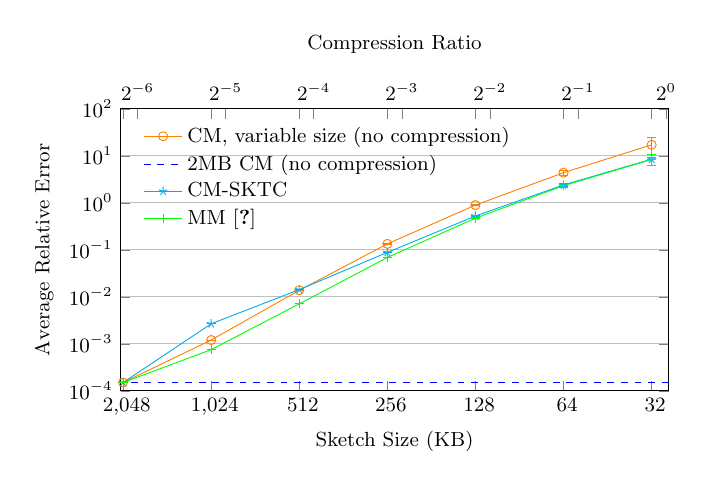
\begin{tikzpicture}[font=\small, scale=\myScale]

\begin{axis}[
        scale only axis,
        xlabel={Sketch Size (KB)},
        ylabel={Average Relative Error},
        xmode=log,
        log basis x=2,
        ymode=log,
        log basis y=10,
        ytick={0.0001,0.001,0.01,0.1,1,10,100},
        % log ticks with fixed point,
        xmin=28,
        xmax=2090,
        ymin= 0.0001,
        ymax = 100,
        ymajorgrids,
        x dir=reverse,
        xticklabel={
        \pgfkeys{/pgf/fpu=true}
        \pgfmathparse{int(2^\tick)}
        \pgfmathprintnumber[fixed]{\pgfmathresult}
        },
        height = 2*0.18 \columnwidth,
        width = 2*0.35 \columnwidth,
        legend style={at={(0.38,0.97)},anchor=north, draw=none, fill=none},
        legend cell align={left}
    ]
    

    \addplot[color=orange, mark=o, error bars/.cd, y dir=both, y explicit relative] coordinates {
        (32,17.2301386655751)+=(32,0.456273716855175)-=(32,0.456273716855175)
        (64,4.39851276684124)+=(64,0.125194135451736)-=(64,0.125194135451736)
        (128,0.897817799438924)+=(128,0.0331188667190209)-=(128,0.0331188667190209)
        (256,0.134055977504855)+=(256,0.0101784884960035)-=(256,0.0101784884960035)
        (512,0.0137905579843333)+=(512,0.00258244268887848)-=(512,0.00258244268887848)
        (1024,0.00120311464471896)+=(1024,0.000617359130580432)-=(1024,0.000617359130580432)
        (2048,0.000149737707752551)+=(2048,0.000271013920590392)-=(2048,0.000271013920590392)
    };
    \addlegendentry{CM, variable size (no compression)}
    
    \addplot [color=blue, domain=28:2090, dashed] {0.000149737707752551};
    \addlegendentry{2MB CM (no compression)}
    \addplot[color=cyan, mark=star, error bars/.cd, y dir=both, y explicit relative] coordinates {
        (32,8.50763586140085)+=(32,0.260338789864091)-=(32,0.260338789864091)
        (64,2.41233720425902)+=(64,0.0811565432460121)-=(64,0.0811565432460121)
        (128,0.524980932282619)+=(128,0.0282927869416904)-=(128,0.0282927869416904)
        (256,0.0883494285351726)+=(256,0.00848242056753894)-=(256,0.00848242056753894)
        (512,0.0142551949578031)+=(512,0.00276276859634349)-=(512,0.00276276859634349)
        (1024,0.00267072482933362)+=(1024,0.00102240698590769)-=(1024,0.00102240698590769)
        (2048,0.000149737707752551)+=(2048,0.000271013920590392)-=(2048,0.000271013920590392)
    };
    \addlegendentry{CM-SKTC}

    \addplot[color=green, mark=+, error bars/.cd, y dir=both, y explicit relative] coordinates {
        (32,8.39710896896061)+=(32,0.265442012913497)-=(32,0.265442012913497)
        (64,2.32340612291331)+=(64,0.0785598660178268)-=(64,0.0785598660178268)
        (128,0.473333620715826)+=(128,0.023338511940957)-=(128,0.023338511940957)
        (256,0.0688385614051386)+=(256,0.00833248009924655)-=(256,0.00833248009924655)
        (512,0.00708697096724866)+=(512,0.00213546569353468)-=(512,0.00213546569353468)
        (1024,0.000751364202893397)+=(1024,0.000553457068376218)-=(1024,0.000553457068376218)
        (2048,0.000149737707752551)+=(2048,0.000271013920590392)-=(2048,0.000271013920590392)
    };
    \addlegendentry{MM~\cite{yang2018elastic}}
    
    
\end{axis}
\begin{axis}[
  scale only axis,
  xlabel={Compression Ratio},
    x label style={at={(axis description cs:0.5,1.29)},anchor=north},
  xmin=28/2048,xmax=2090/2048,
  xmode=log,
  log basis x=2,
  ymin= 0.001,
  ymax = 100,
  axis y line=none,
  axis x line*=top,
  %xticklabels={$1$, $1$, $1/2$, $1/4$, $1/8$, $1/16$, $1/32$, $1/64$},
  height = 2*0.18 \columnwidth,
  width = 2*0.35 \columnwidth,]
\end{axis}
\end{tikzpicture}
\caption{Single node: Compression methods comparison}\label{sktc-fig:general-method-comparison}
\end{figure}

Figure \ref{sktc-fig:general-method-comparison} compares the different compression methods for different sketch sizes. The blue-dashed baseline represents the \textit{ARE} of the 2 MB CM sketch that both compression methods initiate from. One can observe that CM-SKTC outperforms the two other methods consistently. Furthermore, as the compression ratio decreases and the summary size increases, the \textit{ARE} improves, as expected.

\begin{figure}[!htb]
\centering
% This file was created by tikzplotlib v0.8.7.
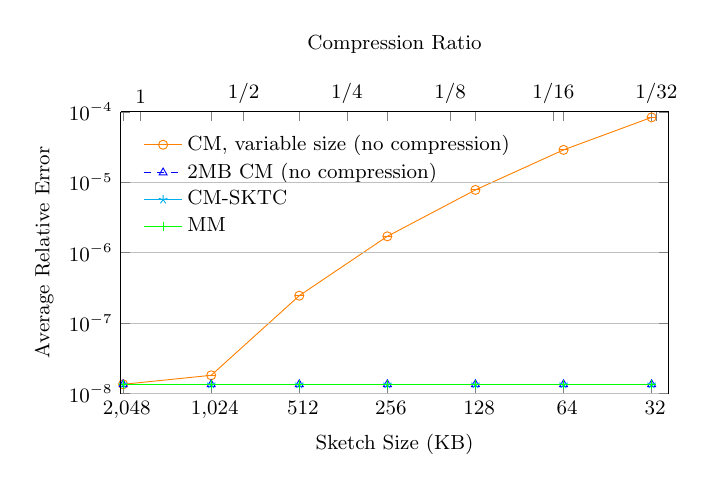
\begin{tikzpicture}[font=\small, scale=\myScale]

\begin{axis}[
        scale only axis,
        xlabel={Sketch Size (KB)},
        ylabel={Average Relative Error},
        xmode=log,
        log basis x=2,
        ymode=log,
        log basis y=10,
        xmin=28,
        xmax=2090,
        ymin= 10e-8,
        ymax = 10e-3,
        ymajorgrids,
        axis y line=none,
        log ticks with fixed point,
        x dir=reverse,
        xticklabel={
        \pgfkeys{/pgf/fpu=true}
        \pgfmathparse{int(2^\tick)}
        \pgfmathprintnumber[fixed]{\pgfmathresult}
        },
        height = 2*0.18 \columnwidth,
        width = 2*0.35 \columnwidth,
        legend style={at={(0.38,0.95)},anchor=north, draw=none, fill=none},
        legend cell align={left}
    ]
    
    %Change this line to single line without points (Also Figure 5), extend to 2048
    
    \addplot[color=orange, mark=o, error bars/.cd, y dir=both, y explicit relative] coordinates {
(32,0.00795579363029106)+=(32,0.00162895737328799)-=(32,0.00162895737328799)
(64,0.00210953168746669)+=(64,0.000599802582637658)-=(64,0.000599802582637658)
(128,0.000411176282548868)+=(128,0.000137097717563645)-=(128,0.000137097717563645)
(256,6.17486343494554E-05)+=(256,5.21386879346016E-05)-=(256,5.21386879346016E-05)
(512,5.45813819295529E-06)+=(512,1.28323308856708E-05)-=(512,1.28323308856708E-05)
(1024,2.11168238388759E-07)+=(1024,9.04130906579136E-07)-=(1024,9.04130906579136E-07)
(2048,0.000000146090104)+=(2048,5.91256371062124E-07)-=(2048,5.91256371062124E-07)
    };
    \addlegendentry{CM, variable size (no compression)}
    
    \addplot[color=blue, dashed, mark=triangle ,mark options={solid}] coordinates {
        (32,0.000000146090104) += (32,0.000271013920590392) -= (32,0.000271013920590392)
        (64,0.000000146090104) += (64,0.000271013920590392) -= (64,0.000271013920590392)
        (128,0.000000146090104) += (128,0.000271013920590392) -= (128,0.000271013920590392)
        (256,0.000000146090104) += (256,0.000271013920590392) -= (256,0.000271013920590392)
        (512,0.000000146090104) += (512,0.000271013920590392) -= (512,0.000271013920590392)
        (1024,0.000000146090104) += (1024,0.000271013920590392) -= (1024,0.000271013920590392)
        (2048,0.000000146090104) += (2048,0.000271013920590392) -= (2048,0.000271013920590392)
    };
    \addlegendentry{2MB CM (no compression)}
    
    \addplot[color=cyan, mark=star, error bars/.cd, y dir=both, y explicit relative] coordinates {
        (32,0.000000146090104) += (32,0.000271013920590392) -= (32,0.000271013920590392)
        (64,0.000000146090104) += (64,0.000271013920590392) -= (64,0.000271013920590392)
        (128,0.000000146090104) += (128,0.000271013920590392) -= (128,0.000271013920590392)
        (256,0.000000146090104) += (256,0.000271013920590392) -= (256,0.000271013920590392)
        (512,0.000000146090104) += (512,0.000271013920590392) -= (512,0.000271013920590392)
        (1024,0.000000146090104) += (1024,0.000271013920590392) -= (1024,0.000271013920590392)
        (2048,0.000000146090104) += (2048,0.000271013920590392) -= (2048,0.000271013920590392)
    };
    \addlegendentry{CM-SKTC}

    \addplot[color=green, mark=+, error bars/.cd, y dir=both, y explicit relative] coordinates {
        (32,0.000000146090104) += (32,0.000271013920590392) -= (32,0.000271013920590392)
        (64,0.000000146090104) += (64,0.000271013920590392) -= (64,0.000271013920590392)
        (128,0.000000146090104) += (128,0.000271013920590392) -= (128,0.000271013920590392)
        (256,0.000000146090104) += (256,0.000271013920590392) -= (256,0.000271013920590392)
        (512,0.000000146090104) += (512,0.000271013920590392) -= (512,0.000271013920590392)
        (1024,0.000000146090104) += (1024,0.000271013920590392) -= (1024,0.000271013920590392)
        (2048,0.000000146090104) += (2048,0.000271013920590392) -= (2048,0.000271013920590392)
    };
    \addlegendentry{MM}
    
    
\end{axis}
\begin{axis}[
  scale only axis,
  xlabel={Compression Ratio},
  ylabel={Average Relative Error},
  x label style={at={(axis description cs:0.5,1.3)},anchor=north},
  xmin=28/2048,xmax=1111/2048,
  xmode=log,
  log basis x=2,
  ymode=log,
ymin= 10e-9,
ymax = 10e-5,
ymajorgrids,
  axis x line*=top,  
  xticklabels={$1$, $1$, $1/2$, $1/4$, $1/8$, $1/16$, $1/32$, $1/64$},
  ytick={0.0001,0.00001, 0.000001, 0.0000001, 0.00000001},
  height = 2*0.18 \columnwidth,
  width = 2*0.35 \columnwidth,]
\end{axis}
\end{tikzpicture}

\caption{Single node: Compression methods comparison - top 50 flows. The 2MB-CM, CM-SKTC, and MM lines coalesce.}\label{sktc-fig:top50-method-comparison}
\end{figure}

In Figure \ref{sktc-fig:top50-method-comparison} we depict the same comparison as Figure \ref{sktc-fig:general-method-comparison}; however we choose a larger sample size of flows, and only to the 50 largest flows \textit{ARE} in each trace are considered. In this graph, one can observe that the top flows \textit{ARE} is extremely low for all methods. Moreover, the MM and CM-SKTC curves are similar, and both have the same error as the 2MB sketch.


%In Table \ref{sktc-table:evaluation:running_times} we compare the time of both the compression process and the query of the MM and CM-SKTC compression.
\inblue{Note that,} the MM is more time-efficient than the CM-SKTC compression. This is due to each hash being calculated twice (for the insertion and for the compression), and therefore we expect the CM-SKTC to be roughly twice as slow as the MM. \inred{Table~\ref{sktc-table:evaluation:data-sent} shows that our compression scheme has a lower packet overhead than MM. While MM may be faster, we can reduce the bandwidth used by the sketch significantly.}

From Figures \ref{sktc-fig:general-method-comparison} and \ref{sktc-fig:top50-method-comparison}, we deduce that the CM-SKTC has two important traits: (1) CM-SKTC achieves estimations within the required error parameters using smaller summaries, and (2) For large (elephant) flows this error is negligible.

\subsection{TA-CM with two ingestion nodes ($n=2$)}
\label{sktc-ssc:eval:TA-CM:2}
We now simulate two local nodes receiving a data stream of size $N$, where the relation between the size of the data stream $N_1$ processed at the first node, and the size of the data stream $N_2$ at the second node is $k=\frac{N_1}{N_2}$. We evaluate the effect of $k$ on the \textit{ARE}. 

Figure \ref{sktc-fig:two-servers-distribution} depicts the \textit{ARE} of merging two sketches when sending different sizes over the network. We compare locally building two sketches with error $\epsilon$, such that they each have size $1$MB (meaning $2$MB of data is sent over the network), and building larger local sketches with error $\sigma \epsilon$ and compressing them. We compare the trivial compression by factor $1 / \sigma$ compared to using our optimal resize factors, for $\sqrt{k}=3,7,10$. Note that our comparison shows that the error of resizing using optimal factors falls in between the error of starting with error $\epsilon$ and trivially compressing with error $\sigma \epsilon$. Of great importance is that even in the worst case the error is less than $\epsilon$. Table \ref{sktc-table:evaluation:data-sent} compares the summaries size across the network. It follows that there is a trade-off between the accuracy and the summaries size.
Figure \ref{sktc-fig:data-sent-ratio} shows the ratio between summaries size as a function of $k$, in relation to trivial compression.

\begin{figure}[!t]
\centering
% This file was created by tikzplotlib v0.8.7.
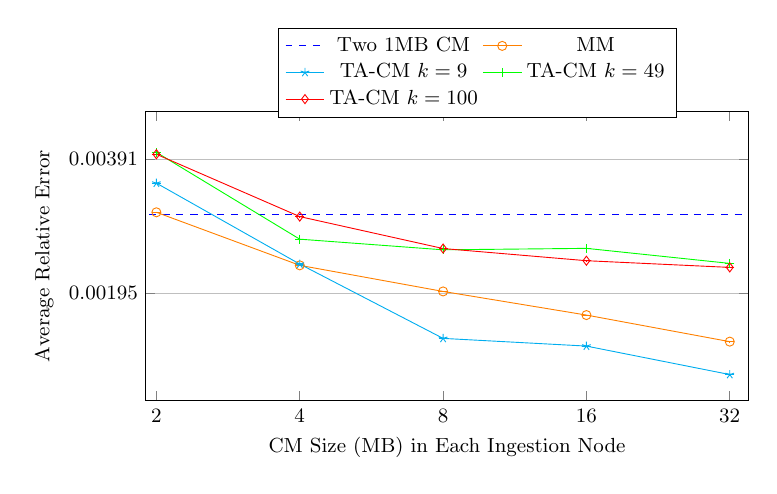
\begin{tikzpicture}[font=\small, scale=\myScale]

\begin{axis}[
        xlabel={CM Size (MB) in Each Ingestion Node},
        ylabel={Average Relative Error},
        xmode=log,
        log basis x=2,
        ymode=log,
        log basis y=2,
        log ticks with fixed point,
        xmin=1.9,
        xmax=35,
        ymin= 0,
        ymax = 0.005,
        ymajorgrids,
        height = 2*0.25 \columnwidth,
        width = 2*0.45 \columnwidth,
        legend style={at={(0.55,1.29)},anchor=north},
        legend columns = 2
        legend width = 2*0.35
        % mark repeat=5,
    ]
    
    \addplot [color=blue, domain=1:35, dashed] {0.002931419};
    \addlegendentry{Two 1MB CM}

    \addplot[color=orange, mark=o, error bars/.cd, y dir=both, y explicit relative] coordinates {
        (2,0.00296915803480048)+=(2,0.000347110578138022)-=(2,0.000347110578138022)
        (4,0.002256303092097967)+=(4,0.000358129292794643)-=(4,0.000358129292794643)
        (8,0.001971592412154686)+=(8,0.000367505249328563)-=(8,0.000367505249328563)
        (16,0.0017443431490592135)+=(16,0.000369607765498873)-=(16,0.000369607765498873)
        (32,0.001520224889699387)+=(32,0.000448184951568447)-=(32,0.000448184951568447)
    };
    \addlegendentry{MM}
    
    \addplot[color=cyan, mark=star, error bars/.cd, y dir=both, y explicit relative] coordinates {
        (2,0.0034529583824306)+=(2,0.000859556663510899)-=(2,0.000859556663510899)
        (4,0.00227091006184114)+=(4,0.00108749299593454)-=(4,0.00108749299593454)
        (8,0.00154598340803716)+=(8,0.000473362436844997)-=(8,0.000473362436844997)
        (16,0.00148559916036538)+=(16,0.000431282460768933)-=(16,0.000431282460768933)
        (32,0.00128208372348584)+=(32,0.0003850265319484)-=(32,0.0003850265319484)
    };
    \addlegendentry{TA-CM $k=9$}
    
    \addplot[color=green, mark=+, error bars/.cd, y dir=both, y explicit relative] coordinates {
        (2,0.00404911795243449)+=(2,0.000949957428845652)-=(2,0.000949957428845652)
        (4,0.00258340366490199)+=(4,0.000740916941009595)-=(4,0.000740916941009595)
        (8,0.00244495913594148)+=(8,0.00056656960414439)-=(8,0.00056656960414439)
        (16,0.00246352697587617)+=(16,0.000733011180075582)-=(16,0.000733011180075582)
        (32,0.00227907488232002)+=(32,0.000563417808543281)-=(32,0.000563417808543281)
    };
    \addlegendentry{TA-CM $k=49$}
    
    \addplot[color=red, mark=diamond, error bars/.cd, y dir=both, y explicit relative] coordinates {
(2,0.00400958809069177)+=(2,0.000782754740222883)-=(2,0.000782754740222883)
(4,0.00290372943567313)+=(4,0.000722232777089102)-=(4,0.000722232777089102)
(8,0.00246138051393235)+=(8,0.000502715484257819)-=(8,0.000502715484257819)
(16,0.00231092449094757)+=(16,0.000808776961871573)-=(16,0.000808776961871573)
(32,0.00223232953999738)+=(32,0.000394832438639461)-=(32,0.000394832438639461)
    };
    \addlegendentry{TA-CM $k=100$}
    
\end{axis}
\end{tikzpicture}

\caption{Two nodes: Compression methods comparison}\label{sktc-fig:two-servers-distribution}

\end{figure}

\begin{figure}[!t]
\centering
% This file was created by tikzplotlib v0.8.7.
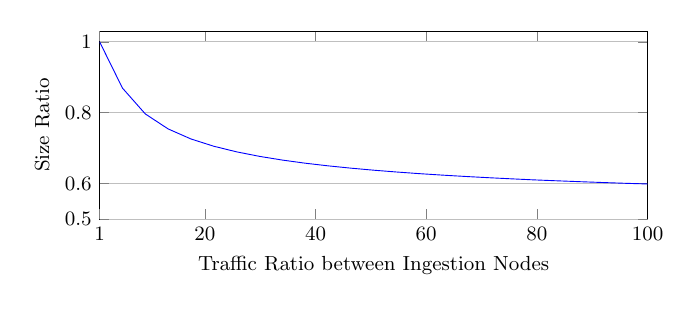
\begin{tikzpicture}[font=\small, scale=\myScale]

\begin{axis}[
        scale only axis,
        xlabel={Traffic Ratio between Ingestion Nodes},
        ylabel={Size Ratio},
        log ticks with fixed point,
        xmin=1,
        xmax=100,
        ymin= 0.5,
        ymax = 1.03,
        ymajorgrids,
        height = 0.24 \columnwidth,
        width = 2*0.35 \columnwidth,
        legend style={at={(0.8,0.6)},anchor=north, draw=none},
        extra x ticks ={1},
        extra y ticks ={0.5},
    ]
    
    \addplot+[blue, mark=none,domain=1:100] {(x^(1/2)+1)^2)/(2*(x+1)};
\end{axis}
\end{tikzpicture}
\caption{Ratio between summaries size in multiple compression methods 
}\label{sktc-fig:data-sent-ratio}
\end{figure}

\begin{table}[!t]
\caption{Compression Ratio by $k$ \label{sktc-table:evaluation:data-sent}}
    \centering
	\begin{tabular}{|c|c|}
	    \hline
		 \textbf{\shortstack{Compression \\ Method}}  & \textbf{\shortstack{Summaries Size Sent \\ (\% from max)}} \\ 
		\hline
		Maximum Merging & 2 MB (100\%)  \\ 
		\hline
		TA-CM, $k=1$ & 2 MB (100\%)  \\ 
		\hline
		TA-CM, $k=9$ & 1.6 MB (80\%)  \\ 
		\hline
		TA-CM, $k=49$ & 1.28 MB (64.3\%)  \\ 
		\hline
		TA-CM, $k=100$ & 1.18 MB (59\%)  \\ 
		\hline
	\end{tabular}
	 
%	\vspace{-6mm}
\end{table}

In Figure \ref{sktc-fig:two-servers-distribution-2MB} we show the results of compressing the same base CM sketch as in Figure \ref{sktc-fig:two-servers-distribution}. However, in this simulation, we compare the results when the total summaries size is $2$MB, i.e., the summaries account for $2$MB of network traffic. In this case, we observe that the TA-CM \textit{ARE} is better than the MM \textit{ARE}. TA-CM outperforms MM as it is traffic-aware and considers the distribution across the nodes and calculates the ratios accordingly; it helps to send the larger part of the data from the node that handled the larger chunk of the stream.

\begin{figure}[!t]
\centering
% This file was created by tikzplotlib v0.8.7.
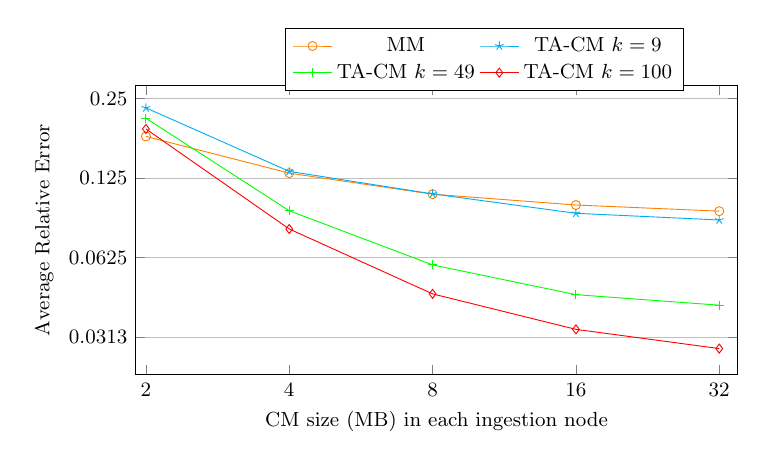
\begin{tikzpicture}[font=\small, scale=\myScale]

\begin{axis}[
        xlabel={CM size (MB) in each ingestion node},
        ylabel={Average Relative Error},
        xmode=log,
        log basis x=2,
        ymode=log,
        log basis y=2,
        log ticks with fixed point,
        xmin=1.9,
        xmax=35,
        ymin= 0,
        ymax = 0.28,
        ymajorgrids,
        height = 2*0.25 \columnwidth,
        width = 2*0.45 \columnwidth,
        legend style={at={(0.58,1.20)},anchor=north},
        legend columns = 2
        legend width = 2*0.35 \columnwidth,
        % mark repeat=5,
    ]
    
    \addplot[color=orange, mark=o] coordinates {
        (2,0.179743449)
        (4,0.130527461)
        (8,0.108661266)
        (16,0.098897622)
        (32,0.093743353)
    };
    \addlegendentry{MM}
    
    \addplot[color=cyan, mark=star] coordinates {
        (2,0.230504062225623)
        (4,0.13258234871128)
        (8,0.108942408575435)
        (16,0.0920066621666375)
        (32,0.0867979682007765)
    };
    \addlegendentry{TA-CM $k=9$}
    
    \addplot[color=green, mark=+] coordinates {
        (2,0.210633144817792)
        (4,0.0940809172884923)
        (8,0.0586891464861655)
        (16,0.0452908789372009)
        (32,0.0413224013064837)
    };
    \addlegendentry{TA-CM $k=49$}
    
    \addplot[color=red, mark=diamond] coordinates {
        (2,0.191880649575314)
        (4,0.0802466257250163)
        (8,0.0455919938550279)
        (16,0.0334732122784799)
        (32,0.0283161105139431)
    };
    \addlegendentry{TA-CM $k=100$}
    
\end{axis}
\end{tikzpicture}

\caption{Two nodes: Compression methods comparison. Allowance of $2$MB sent from ingestion nodes to centralized server.} \label{sktc-fig:two-servers-distribution-2MB}

\end{figure}

\subsection{TA-CM with $n$ ingestion nodes}
\label{sktc-ssc:eval:TA-CM:n}
\begin{figure}[!htb]
\centering

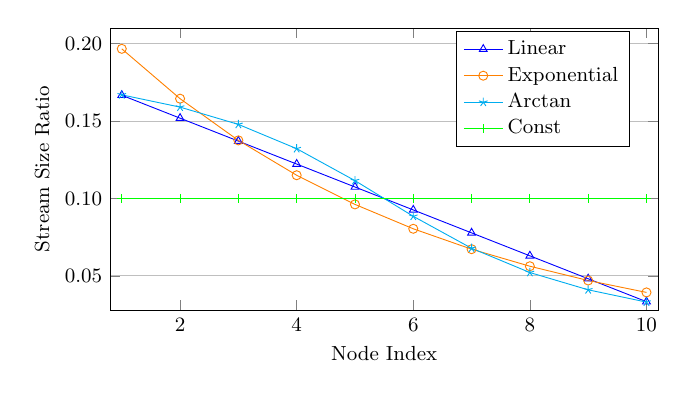
\begin{tikzpicture}[font=\small, scale=\myScale]

\begin{axis}[
        scale only axis,
        xlabel={Node Index},
        ylabel={Stream Size Ratio},
        xmin=0.8,
        xmax=10.2,
        ymin= 0.028,
        ymax = 0.21,
        ymajorgrids,
        yticklabel=\pgfkeys{/pgf/number format/.cd,fixed,precision=2,zerofill}\pgfmathprintnumber{\tick},
        height = 2*0.18 \columnwidth,
        width = 2*0.35 \columnwidth,
        legend style={at={(0.79,0.99)},anchor=north},
        legend cell align={left}
    ]
    %add ticks all x
    \addplot[color=blue, mark=triangle] coordinates {
        (1,0.166666667)
        (2,0.151851852)
        (3,0.137037037)
        (4,0.122222222)
        (5,0.107407407)
        (6,0.092592593)
        (7,0.077777778)
        (8,0.062962963)
        (9,0.048148148)
        (10,0.033333333)
    };
    \addlegendentry{Linear}

    \addplot[color=orange, mark=o] coordinates {
        (1,0.196636457)
        (2,0.16443744)
        (3,0.137510979)
        (4,0.114993698)
        (5,0.096163598)
        (6,0.080416908)
        (7,0.067248722)
        (8,0.056236813)
        (9,0.047028093)
        (10,0.039327291)
    };
    \addlegendentry{Exponential}
    
    \addplot[color=cyan, mark=star] coordinates {
        (1,0.16692565)
        (2,0.1589913)
        (3,0.14783371)
        (4,0.13215652)
        (5,0.11151949)
        (6,0.0884805)
        (7,0.06784347)
        (8,0.05216628)
        (9,0.04100869)
        (10,0.033074344)
    };
    \addlegendentry{Arctan}
    
    \addplot[color=green, mark=+] coordinates {
        (1,0.1)
        (2,0.1)
        (3,0.1)
        (4,0.1)
        (5,0.1)
        (6,0.1)
        (7,0.1)
        (8,0.1)
        (9,0.1)
        (10,0.1)
    };
    \addlegendentry{Const}
    
\end{axis}
\end{tikzpicture}
\caption{$n=10$ nodes: Stream size distribution over the nodes}\label{sktc-fig:10-servers-distribution}
\end{figure}

To evaluate TA-CM in multiple-ingestion nodes scenarios, we formulate four different types of distributions for 10 nodes (see Figure \ref{sktc-fig:10-servers-distribution}) and compare the TA-CM to MM and the non-compressed CM sketch. The distributions were chosen such that the ratio between the largest server ratio to the smallest server ratio is 5 (i.e., $N_1 / N_{10} = 5$).

The  CM sketch base size for each of the $10$ nodes is $32$KB. We compare the \textit{ARE} with multiple values of $\sigma$ (i.e., the ratio by which the ingestion node CM sizes is increased) and compressing with two methods: (1) TA-CM with ratios computed in Section \ref{sktc-sec:resize} (2) MM compression with all ratios are $1/\sigma$. As depicted in Figure~\ref{sktc-fig:10-servers-distribution-compression}, TA-CM achieves similar results in terms of \textit{ARE} to the Maximum Merging compression and improves the results of the basic non-compressed CM. However, it does so while decreasing the total summaries size.  Table \ref{sktc-table:evaluation:cr-distributions} indicates that the TA-CM saves between 7\% to 9\% of the total summaries size for chosen distributions. This saving ratio can be increased by choosing other, wider distributions of the stream (for example if the stream distributes across the ingestion nodes by Pareto distribution then TA-CM potentially saves an even higher percentage).

\begin{table}[!htb]
	\caption{Compression ratio of various distributions}

    \centering
	\begin{tabular}{|c|c|}
	    \hline
		\textbf{Distribution}  & \textbf{\shortstack{Summaries Size \\ (\% from max)}} \\ 
		\hline
		Maximum Merging & 320KB (100\%)  \\ 
		\hline
		Constant Dist. & 320KB (100\%)  \\ 
		\hline
		Exponential Dist. & $\sim$ 292KB (91.3\%)  \\ 
		\hline
		Linear Dist. & $\sim$ 298KB (93.3\%)  \\ 
		\hline
		Arctan Dist. & $\sim$ 293KB (91.6\%)  \\ 
		\hline
	\end{tabular}
	\label{sktc-table:evaluation:cr-distributions}
%	\vspace{-6mm}
\end{table}

\begin{figure}[!htb]
\centering

% This file was created by tikzplotlib v0.8.7.
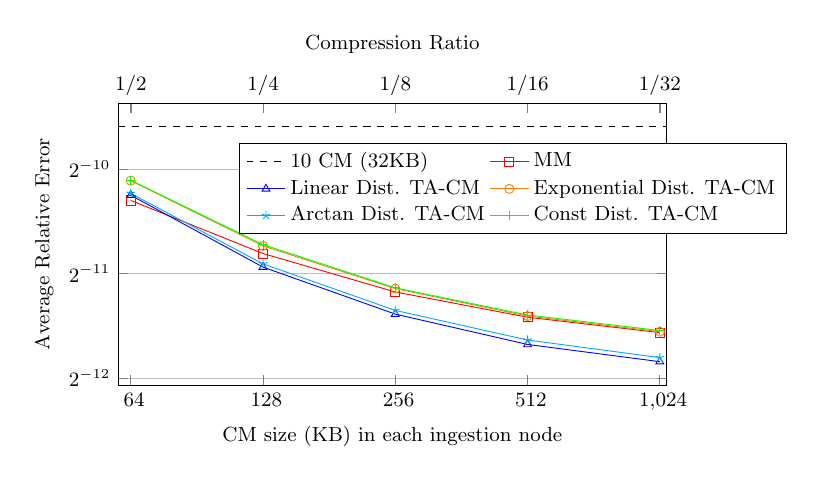
\begin{tikzpicture}[font=\small, scale=\myScale]

\begin{axis}[
        scale only axis,
        xlabel={CM size (KB) in each ingestion node},
        ylabel={Average Relative Error},
        xmode=log,
        log basis x=2,
        ymode=log,
        log basis y=2,
        xmin=60,
        xmax=1060,
        log ticks with fixed point,
        height = 2*0.18 \columnwidth,
        width = 2*0.35 \columnwidth,
        yticklabels={$2^{-13}$,$2^{-12}$, $2^{-11}$, $2^{-10}$},
        ymajorgrids,
        xticklabel={
        \pgfkeys{/pgf/fpu=true}
        \pgfmathparse{int(2^\tick)}
        \pgfmathprintnumber[fixed]{\pgfmathresult}
        },
        legend style={at={(0.72,0.86)},anchor=north},
        legend columns = 2,
        legend cell align={left}
    ]
    
    %change to fixed line
    \addplot [color=black, domain=60:1060, dashed] {0.001295165};
    \addlegendentry{10 CM (32KB)}

    \addplot[color=red, mark=square] coordinates {
        (64,0.000794505)
        (128,0.000558492)
        (256,0.000432703)
        (512,0.00036593)
        (1024,0.000330449)
    };
    \addlegendentry{MM}
    
    \addplot[color=blue, mark=triangle] coordinates {
        (64,0.000822598)
        (128,0.000510391)
        (256,0.000373544)
        (512,0.000305408)
        (1024,0.00027242)
    };
    \addlegendentry{Linear Dist. TA-CM}
    
    \addplot[color=orange, mark=o] coordinates {
        (64,0.000905932)
        (128,0.000587575)
        (256,0.000442481)
        (512,0.000368815)
        (1024,0.000332426)
    };
    \addlegendentry{Exponential Dist. TA-CM}
    
    \addplot[color=cyan, mark=star] coordinates {
        (64,0.000832502)
        (128,0.000521449)
        (256,0.000382919)
        (512,0.000314548)
        (1024,0.000279836)
    };
    \addlegendentry{Arctan Dist. TA-CM}
    
    \addplot[color=green, mark=+] coordinates {
        (64,0.000908105)
        (128,0.000592652)
        (256,0.000444668)
        (512,0.000371463)
        (1024,0.000335038)
    };
    \addlegendentry{Const Dist. TA-CM}
    
\end{axis}
\begin{axis}[
  scale only axis,
  xlabel={Compression Ratio},
    x label style={at={(axis description cs:0.5,1.27)},anchor=north},
  xmin=60/2048,xmax=1060/2048,
  xmode=log,
  log basis x=2,
  ymin= 0.001,
  ymax = 100,
  axis y line=none,
  axis x line*=top,
  xticklabels={$1$, $1/2$, $1/4$, $1/8$, $1/16$, $1/32$},
  height = 2*0.18 \columnwidth,
  width = 2*0.35 \columnwidth,]
\end{axis}

\end{tikzpicture}

\caption{$n=10$ nodes: Compression method comparison - various distributions}\label{sktc-fig:10-servers-distribution-compression}
\end{figure}

\subsection{TA-KMV with $n$ ingestion nodes}\label{sktc-subsec:eval:kmv}
%Replace the word record
%replace the word number with # in X labels
In this section, we evaluate \emph{TA-KMV}. We use the same method as in the previous section to generate the input stream. However, for this section, we use only the linear distribution. We compare our \emph{TA-KMV} with multiple compression ratios. The compression ratio is measured by \emph{Total Hash-values Sent (THS)}. To the best of our knowledge, no compression scheme is available for this sketch, and therefore we compare our method only to the baseline, i.e., each ingestion node sends $k$ hash values to the centralized server. Our measurement unit is the estimation precision rate to true cardinality. In this case, the number of hash values that are sent to the centralized server is $n \cdot k$, where $n$ is the number of ingestion nodes.

\begin{figure}[!htb]
\centering

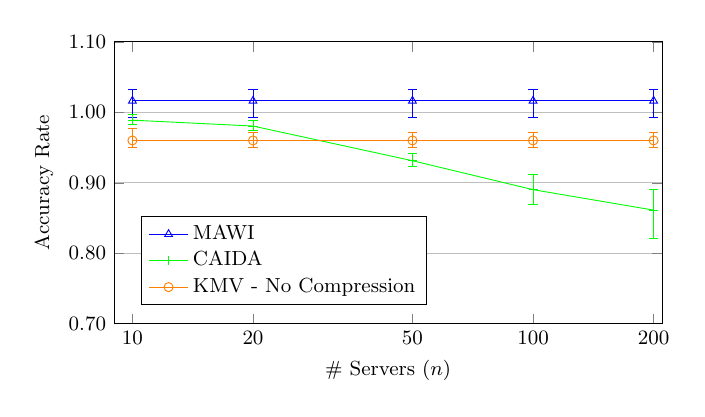
\begin{tikzpicture}[font=\small, scale=\myScale]

\begin{axis}[
        scale only axis,
        xlabel={\# Servers ($n$)},
        ylabel={Accuracy Rate},
        xmin=9,
        xmax=210,
        ymin= 0.70,
        ymajorgrids,
        ymax = 1.1,
        xmode=log,
        log ticks with fixed point,
        xtick = {5,10,20,50,100,200},
        yticklabel=\pgfkeys{/pgf/number format/.cd,fixed,precision=2,zerofill}\pgfmathprintnumber{\tick},
        height = 2*0.18 \columnwidth,
        width = 2*0.35 \columnwidth,
        legend style={at={(0.05,0.065)},anchor=south west},
        legend cell align={left}
    ]
    
    \addplot[color=blue, mark=triangle, error bars/.cd, y dir=both, y explicit relative] coordinates {
(10,1.01612079900443)  += (10,0.0157908595664422) -=(10,0.0224356127165992)
(20,1.01612079900443)  += (20,0.0162978598619865) -=(20,0.0224356127165992)
(50,1.01612079900443)  += (50,0.0162978598619865) -=(50,0.0224356127165992)
(100,1.01612079900443)  += (100,0.0162978598619865) -=(100,0.0224356127165992)
(200,1.01612079900443)  += (200,0.0162978598619865) -=(200,0.0224356127165992)
    };
    \addlegendentry{MAWI}
    
    \addplot[color=green, mark=+, error bars/.cd, y dir=both, y explicit relative] coordinates {
(10,0.988813459783557)  += (10,0.00800539555909119) -=(10,0.00595529407844508)
(20,0.980463796203664)  += (20,0.00830907805368898) -=(20,0.00658938198094061)
(50,0.931249963187018)  += (50,0.0109794749801466) -=(50,0.00797865392094566)
(100,0.890186318982447)  += (100,0.0235224353515718) -=(100,0.0234221082610149)
(200,0.861126139373611)  += (200,0.0342711777766666) -=(200,0.0462573349075841)
    };
    \addlegendentry{CAIDA}
    
    \addplot[color=orange, mark=o, error bars/.cd, y dir=both, y explicit relative] coordinates {
(10,0.960038171361342)  += (10,0.0174336347135434) -=(10,0.0110330067979534)
(20,0.960038171361342)  += (20,0.0124716598206064) -=(20,0.0110330067979534)
(50,0.960038171361342)  += (50,0.0124716598206064) -=(50,0.0110330067979534)
(100,0.960038171361342)  += (100,0.0124716598206064) -=(100,0.0110330067979534)
(200,0.960038171361342)  += (200,0.0124716598206064) -=(200,0.0110330067979534)
    };
    \addlegendentry{KMV - No Compression}
    
\end{axis}

\end{tikzpicture}



\caption{TA-KMV vs baseline for $k=1024$.} \label{sktc-fig:kmv-sktc-eval}
\end{figure}

% \begin{table}[!htb]
% 	\caption{Records sent for various compression methods}

%     \centering
% 	\begin{tabular}{|c|c|}
% 	    \hline
% 		\textbf{Plot}  & \textbf{\shortstack{THS sent for 200 ingestion nodes \\ (\% from max)}} \\ 
% 		\hline
% 		KMV - No Compression & 204800 (100\%)  \\ 
% 		\hline
% 		\emph{TA-KMV, THS}=$k\ln{k}$ & 7498 ( $\sim$ 3.6\%)  \\ 
% 		\hline
% 		\emph{TA-KMV, THS}=$2k\ln{k}$ & 14596 ( $\sim$ 7.1\%)  \\ 
% 		\hline
% 	\end{tabular}
% 	\label{sktc-table:evaluation:sktc-kmv}
% \end{table}

Figure \ref{sktc-fig:kmv-sktc-eval} depicts the impact of the number of ingestion nodes on the accuracy rate of TA-KMV, \inred{with the confidence interval}. We define the accuracy rate as $\frac{\text{Estimation}}{\text{\# Flows}}$. \inblue{The figure shows that the estimation remains fairly accurate even at $100$ nodes. The CAIDA dataset does not have many flows, therefore the aggregate ends up receiving multiples of the same hash value, and thus the \inred{accuracy begins to drop}. For example, at 200 nodes the central server receives only 300 different hash values. Contrast this with MAWI, where, due to the larger number of small flows, the central server receives all 1024 of the smallest hash values. Consider the case of $50$ nodes. The baseline sends $51200$ hash values, whereas the compressed version send around $4150$ hash values -- a $92\%$ decrease for a near negligible decrease in accuracy. This creates a clear trade-off between the accuracy rate and the total summaries size. We note that sending less than $k \ln k$ hash values in total (e.g., $k$) greatly reduced the accuracy of the estimation.}
%In Table \ref{sktc-table:evaluation:sktc-kmv} we show that  although TA-KMV accuracy slightly decreased, it saves more than 90\% of the total hash values sent over the network.
%It allows network operators to decide whether they prefer to lose some accuracy and increase the possible bandwidth over the network, or increase the accuracy and pay more in management packets.


\subsection{TA-HLL with $n$ ingestion nodes}



\label{sktc-ssc:eval:TA-HLL}
Lastly, we compare the  four methods for traffic aware cardinality estimation using compression of distributed HLL described in Section~\ref{sktc-sec:hll}. Recall that the methods are: 

\emph{(i)} (Random) Each node reports each of its counters w.p. $p$.

\emph{(ii)} (Weighted) Reporting a counter value $c$ w.p. $p_c$.

\emph{(iii)} (Largest) Each node reports its  $\beta \cdot m$ largest counters.

\emph{(iv)} (Threshold) Each node reports all its counters with values of at least a threshold $c_T$.

We evaluate the results of these four methods with an HLL array with size 128, using the CAIDA and MAWAI datasets. We evaluate all the four methods through two metrics for accuracy: The first metric is the centralized node Array Recovery Rate given as the percentage of cells in the centralized node recovered array that are identical to the corresponding cells in a HLL sketch that could be computed over all network traffic. The second evaluated metric is the relative error: For a distributed HLL estimation $C$, and real stream cardinality $F$,  the relative error is $RE = \frac{|F-C|}{F}$. We first consider 10 ingestion nodes (and later vary their number).

\begin{figure}[t!]
\centering

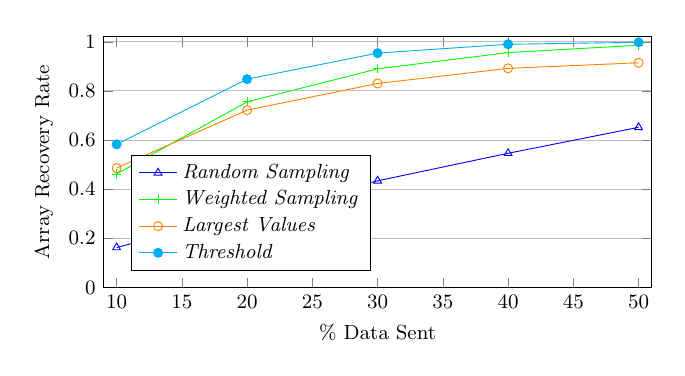
\begin{tikzpicture}[font=\small, scale=\myScale]

\begin{axis}[
        scale only axis,
        xlabel={\% Data Sent},
        ylabel={Array Recovery Rate},
        xmin=9,
        xmax=51,
        ymin= 0,
        ymajorgrids,
        ymax = 1.02,
        height = 2*0.16 \columnwidth,
        width = 2*0.35 \columnwidth,
        legend style={at={(0.05,0.065)},anchor=south west},
        legend cell align={left}
    ]
    
    \addplot[color=blue, mark=triangle, error bars/.cd, y dir=both, y explicit relative] coordinates {
        (10,0.162523674242424)
        (20,0.302260890151515)
        (30,0.434067234848485)
        (40,0.546223958333333)
        (50,0.651811079545455)
    };
    \addlegendentry{\emph{Random Sampling}}
    
    \addplot[color=green, mark=+, error bars/.cd, y dir=both, y explicit relative] coordinates {
        (10,0.46194365530303)
        (20,0.755563446969697)
        (30,0.889973958333333)
        (40,0.956143465909091)
        (50,0.986032196969697)
    };
    \addlegendentry{\emph{Weighted Sampling}}
    
    \addplot[color=orange, mark=o, error bars/.cd, y dir=both, y explicit relative] coordinates {
        (10,0.486100852272727)
        (20,0.721960227272727)
        (30,0.830331439393939)
        (40,0.89188446969697)
        (50,0.914670928030303)
    };
    \addlegendentry{\emph{Largest Values}}
    
    \addplot[color=cyan, mark=*, error bars/.cd, y dir=both, y explicit relative] coordinates {
        (10,0.582682291666667)
        (20,0.848070549242424)
        (30,0.953953598484849)
        (40,0.990056818181818)
        (50,0.998046875)
    };
    \addlegendentry{\emph{Threshold}}
    
\end{axis}

\end{tikzpicture}

\caption{TA-HLL Array Recovery Rate in CAIDA -- 10 ingestion nodes} \label{sktc-fig:eval-hll-arr}
\end{figure}

\begin{figure}[t!]
\centering

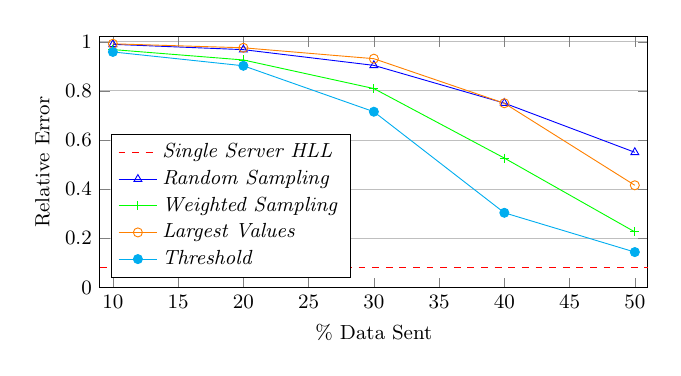
\begin{tikzpicture}[font=\small, scale=\myScale]

\begin{axis}[
        scale only axis,
        xlabel={\% Data Sent},
        ylabel={Relative Error},
        xmin=9,
        xmax=51,
        ymin= 0,
        ymajorgrids,
        ymax = 1.02,
        height = 2*0.16 \columnwidth,
        width = 2*0.35 \columnwidth,
        legend style={at={(0.02,0.04)},anchor=south west},
        legend cell align={left}
    ]
    
    \addplot [color=red, domain=9:210, dashed] {0.081807084};
    \addlegendentry{\emph{Single Server HLL}}
    
    \addplot[color=blue, mark=triangle, error bars/.cd, y dir=both, y explicit relative] coordinates {
        (10,0.989818001815833)
        (20,0.968150415942164)
        (30,0.904137272470303)
        (40,0.750498757765852)
        (50,0.550173699201597)
    };
    \addlegendentry{\emph{Random Sampling}}
    
    \addplot[color=green, mark=+, error bars/.cd, y dir=both, y explicit relative] coordinates {
        (10,0.968407356663112)
        (20,0.926128690744725)
        (30,0.809747424055189)
        (40,0.526700142191625)
        (50,0.226103519616794)
    };
    \addlegendentry{\emph{Weighted Sampling}}
    
    \addplot[color=orange, mark=o, error bars/.cd, y dir=both, y explicit relative] coordinates {
        (10,0.991935446090819)
        (20,0.975726704254263)
        (30,0.931307572956268)
        (40,0.749948665319353)
        (50,0.415925436754393)
    };
    \addlegendentry{\emph{Largest Values}}
    
    \addplot[color=cyan, mark=*, error bars/.cd, y dir=both, y explicit relative] coordinates {
        (10,0.958849167188452)
        (20,0.902461336487268)
        (30,0.715378351707372)
        (40,0.303923157641182)
        (50,0.144018817238216)
    };
    \addlegendentry{\emph{Threshold}}
    
\end{axis}

\end{tikzpicture}



\caption{TA-HLL Relative Error in CAIDA -- 10 ingestion nodes} \label{sktc-fig:eval-hll-re}
\end{figure}





Figure \ref{sktc-fig:eval-hll-arr} shows the Array Recovery Rate for  the four methods, as a function of percentage of data sent across the network as part of all ingestion nodes HLL array sizes. Here, with 10 ingestion nodes and HLL array size of 128, the total size is 1280. 
For instance, 20\% means sending a total of 256 values to the centralized server. 
We can see that methods Weighted sampling (ii) and Threshold (iv) that require an iterative process with the centralized server achieve higher accuracy. 

\begin{figure}[b!]
\centering

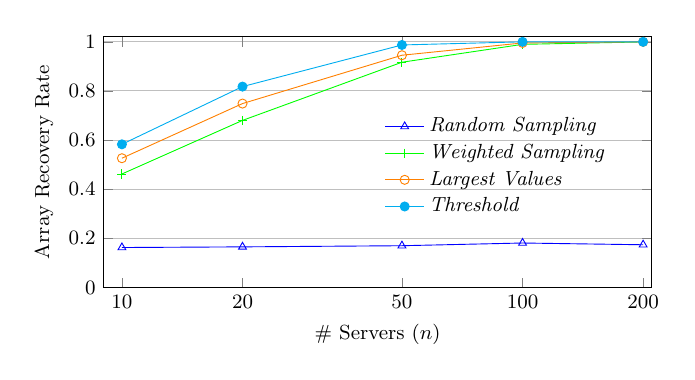
\begin{tikzpicture}[font=\small, scale=\myScale]

\begin{axis}[
        scale only axis,
        xlabel={\# Servers ($n$)},
        ylabel={Array Recovery Rate},
        xmin=9,
        xmax=210,
        ymin= 0,
        ymajorgrids,
        ymax = 1.02,
        xmode=log,
        log ticks with fixed point,
        xtick = {5,10,20,50,100,200},
        height = 2*0.16 \columnwidth,
        width = 2*0.35 \columnwidth,
        legend style={at={(0.5,0.25)},anchor=south west, draw=none, opacity=1, fill=none},
        legend cell align={left}
    ]
    
    \addplot[color=blue, mark=triangle, error bars/.cd, y dir=both, y explicit relative] coordinates {
        (10,0.162523674242424)
        (20,0.165187026515152)
        (50,0.169862689393939)
        (100,0.180871212121212)
        (200,0.173768939393939)
    };
    \addlegendentry{\emph{Random Sampling}}
    
    \addplot[color=green, mark=+, error bars/.cd, y dir=both, y explicit relative] coordinates {
        (10,0.46194365530303)
        (20,0.680101799242424)
        (50,0.916903409090909)
        (100,0.989701704545455)
        (200,0.999585700757576)
    };
    \addlegendentry{\emph{Weighted Sampling}}
    
    \addplot[color=orange, mark=o, error bars/.cd, y dir=both, y explicit relative] coordinates {
        (10,0.526100852272727)
        (20,0.748579545454545)
        (50,0.945371685606061)
        (100,0.995442708333333)
        (200,0.999881628787879)
    };
    \addlegendentry{\emph{Largest Values}}
    
    \addplot[color=cyan, mark=*, error bars/.cd, y dir=both, y explicit relative] coordinates {
        (10,0.582682291666667)
        (20,0.817708333333333)
        (50,0.987215909090909)
        (100,0.999940814393939)
        (200,1)
    };
    \addlegendentry{\emph{Threshold}}
    
\end{axis}

\end{tikzpicture}



\caption{TA-HLL Array Recovery Rate in CAIDA  -- 10\% data sent} \label{sktc-fig:eval-hll-in-arr}
\end{figure}

\begin{figure}[b!]
\centering

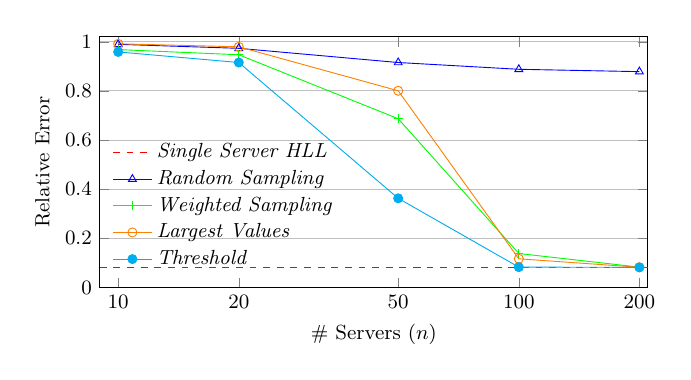
\begin{tikzpicture}[font=\small,scale=\myScale]

\begin{axis}[
        scale only axis,
        xlabel={\# Servers ($n$)},
        ylabel={Relative Error},
        xmin=9,
        xmax=210,
        ymin= 0,
        ymajorgrids,
        ymax = 1.02,
        xmode=log,
        log ticks with fixed point,
        xtick = {5,10,20,50,100,200},
        height = 2*0.16 \columnwidth,
        width = 2*0.35 \columnwidth,
        legend style={at={(0.01,0.04)},anchor=south west, draw=none, opacity=1, fill=none},
        legend cell align={left}
    ]
    
    \addplot [color=red, domain=9:210, dashed] {0.081807084};
    \addlegendentry{\emph{Single Server HLL}}
    
    \addplot[color=blue, mark=triangle, error bars/.cd, y dir=both, y explicit relative] coordinates {
        (10,0.989818001815833)
        (20,0.973515139894837)
        (50,0.91574909464158)
        (100,0.888143415446563)
        (200,0.87856880423703)
    };
    \addlegendentry{\emph{Random Sampling}}
    
    \addplot[color=green, mark=+, error bars/.cd, y dir=both, y explicit relative] coordinates {
        (10,0.968407356663112)
        (20,0.947318190605346)
        (50,0.686897917425959)
        (100,0.138120889057764)
        (200,0.0827054662824469)
    };
    \addlegendentry{\emph{Weighted Sampling}}
    
    \addplot[color=orange, mark=o, error bars/.cd, y dir=both, y explicit relative] coordinates {
        (10,0.991935446090819)
        (20,0.979722025039235)
        (50,0.800648090848471)
        (100,0.116603690823036)
        (200,0.0821491851664647)
    };
    \addlegendentry{\emph{Largest Values}}
    
    \addplot[color=cyan, mark=*, error bars/.cd, y dir=both, y explicit relative] coordinates {
        (10,0.958849167188452)
        (20,0.91577629304402)
        (50,0.36283955355022)
        (100,0.0827209569907977)
        (200,0.081807083923316)
    };
    \addlegendentry{\emph{Threshold}}
    
\end{axis}

\end{tikzpicture}



\caption{TA-HLL Relative Error in CAIDA - 10\% data sent} \label{sktc-fig:eval-hll-in-re}
\end{figure}

\begin{figure}[b!]
\centering

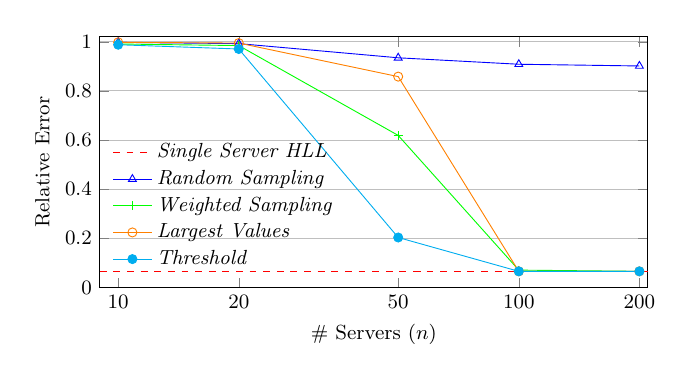
\begin{tikzpicture}[font=\small,scale=\myScale]

\begin{axis}[
        scale only axis,
        xlabel={\# Servers ($n$)},
        ylabel={Relative Error},
        xmin=9,
        xmax=210,
        ymin= 0,
        ymajorgrids,
        ymax = 1.02,
        xmode=log,
        log ticks with fixed point,
        xtick = {5,10,20,50,100,200},
        height = 2*0.16 \columnwidth,
        width = 2*0.35 \columnwidth,
        legend style={at={(0.01,0.04)},anchor=south west, draw=none, opacity=1, fill=none},
        legend cell align={left}
    ]
    
    \addplot [color=red, domain=9:210, dashed] {0.065548765};
    \addlegendentry{\emph{Single Server HLL}}
    
    \addplot[color=blue, mark=triangle, error bars/.cd, y dir=both, y explicit relative] coordinates {
        (10,0.997791172)
        (20,0.992680167)
        (50,0.934956428)
        (100,0.90867773)
        (200,0.901680999)
    };
    \addlegendentry{\emph{Random Sampling}}
    
    \addplot[color=green, mark=+, error bars/.cd, y dir=both, y explicit relative] coordinates {
        (10,0.991108609)
        (20,0.984747064)
        (50,0.61894103)
        (100,0.070554953)
        (200,0.065548765)
    };
    \addlegendentry{\emph{Weighted Sampling}}
    
    \addplot[color=orange, mark=o, error bars/.cd, y dir=both, y explicit relative] coordinates {
        (10,0.998044631)
        (20,0.99495585)
        (50,0.85833174)
        (100,0.065548765)
        (200,0.065548765)
    };
    \addlegendentry{\emph{Largest Values}}
    
    \addplot[color=cyan, mark=*, error bars/.cd, y dir=both, y explicit relative] coordinates {
        (10,0.988117335)
        (20,0.970737772)
        (50,0.203320455)
        (100,0.065548765)
        (200,0.065548765)
    };
    \addlegendentry{\emph{Threshold}}
    
\end{axis}

\end{tikzpicture}

\caption{\inblue{TA-HLL Relative Error in MAWI - 10\% data sent}} \label{sktc-fig:eval-hll-in-re-mawi}
\end{figure}

Figure \ref{sktc-fig:eval-hll-re} presents the relative error of the same scenario, and as one could assume, the two graphs show coordinated results, i.e., the best method in terms of Array Recovery Rate (Threshold) allows lower Relative Error.  
Note that computing the particular threshold values for each node might require a relatively complicated iterative process with the centralized server with potential tradeoff between the number of iterations and communication overhead.
%However, In our simulations we ignored the communication that is needed to find the threshold value to be the correct percentile, in contrary to the Weighted Sampling method, in which we did not ignore the data that sent to the centralized node before the probability calculations. Which means that in realistic scenarios the Weighted Sampling method is possibly better than Threshold method.




In Figures \ref{sktc-fig:eval-hll-in-arr}-\ref{sktc-fig:eval-hll-in-re-mawi}, we present the impact of the number of ingestion nodes across the network on accuracy. We used the same settings as described in previous figures, with only 10\% of the data sent to the centralized node and varied the number of ingestion nodes across the network. Once again the two methods with an iterative process with the centralized server are more accurate than the other two methods. Another observation is that as the number of ingestion nodes increases, the performance improves, that is because the total number of reports that arrive to the centralized node is increasing and as such, the probability to receive per each cell a value identical to that computed for the complete traffic is increasing as well.



\section{Conclusion}\label{sktc-sec:conclusion}
In this paper, we presented the problem of merging data from multiple measurement points to one centralized server, described a distributed traffic-aware sketching scheme, and applied it to three unique sketches. 
We presented the CM-SKTC sketch as a simple, yet efficient method for compressing the CM sketch to any desired size, then used this method to generate \emph{TA-CM}, a new scheme for flow-size measurements that 
%performs as well as previously presented methods 
provides high accuracy 
and  decreases the total summaries size sent to the centralized server by considering the traffic of each node. 
This method is important in today's network design because when the traffic congestion in the network is high the need to successfully measure the network load is higher. In such situations, the extra load created by sending the summaries can worsen network congestion. 

Moreover, we generalized this approach for cardinality estimation and introduced new traffic-aware designs of the KMV sketch as well as of the HLL sketch. They both send fewer values while retaining high accuracy cardinality estimation. 
Finally, we analyzed these sketches under multiple network settings and examined the trade-off between the accuracy and the size of summaries.

Several directions can be the focus in future work.  
%There are some topics we did not address and can be focused on in future work. 
A straightforward extension is developing compression algorithms for additional kinds of sketches %; there are many other types of sketches that 
allowing different measurement tasks (e.g., Quantiles for rank estimation~\cite{agarwal2013mergeable}).  
%Likewise, calculating the TA-KMV compression ratios only takes into account the estimated cardinality at ingestion nodes. It would be interesting to suggest other heuristics for deciding how many (and which) elements to send as part of the summary. For example, we can consider storing the element frequencies alongside the hashes -- as the frequency rises the less likely a node needs to send the specific hash as another node probably has the same element and will send it.
%Moreover, each of the presented compression schemes refers to a sketch supporting a single task such as flow size estimation or cardinality estimation. It is interesting to generalize the approach towards generic sketches such as UnivMon~\cite{liu2016one} and 
%NitroSketch~\cite{NitroSketch} supporting multiple tasks. This might involve definitions for ideal resize factors that refer jointly to multiple tasks, observing different types of errors with potential heterogeneous balance among the required size of summaries for the various nodes.
%Another interesting addition to this paper can be studying the impact of interleaving the ingestion nodes such that streams observed by the nodes might not be disjoint. This problem raises multiple questions related to duplicate handling of the system which we currently ignore by assuming that the ingestion nodes are separate. 
Likewise, we wish to design further compression of sketches 
by leveraging existing generic compression techniques such as Huffman codes, LZ77 or gzip~\cite{huffman1952method, ziv1977universal, deutsch1996gzip}. 

\section{Acknowledgment}
This work was partially supported by the Technion Hiroshi Fujiwara Cyber Security Research Center and the Israel National Cyber Directorate,  
by the Alon fellowship, by German-Israeli Science Foundation (GIF) Young Scientists Program,   
by the Taub Family Foundation as well as  
and by the Polak Fund for Applied Research and by the Gordon Fund for System Engineering, at the Technion. 

\balance
\bibliographystyle{plain}
\bibliography{reference}

\begin{IEEEbiography}
[{\includegraphics[width=1.15in,height=1.42in,clip,keepaspectratio]{Pic_Harris.eps}}]
{Dor Harris} is a PhD candidate at the department of Computer Science of the Technion, Haifa, Israel. He received the BSc in Software Engineering (cum laude) from the Technion in 2014.
\end{IEEEbiography}

\begin{IEEEbiography}
[{\includegraphics[width=1.15in,height=1.42in,clip,keepaspectratio]{Pic_Rinberg.eps}}]
{Arik Rinberg} is a PhD candidate at the department of Electrical and Computer Engineering of the Technion, Haifa, Israel. He received the BSc in Computer Engineering (summa cum laude) from the Technion in 2018.
\end{IEEEbiography}
    


\begin{IEEEbiography}
[{\includegraphics[width=1.15in,height=1.42in,clip,keepaspectratio]{Pic_Rottenstreich.eps}}]
{Ori Rottenstreich} is an assistant professor at the department of Computer Science and the department of Electrical and Computer Engineering of the Technion, Haifa, Israel.  In 2015-2017 he was a Postdoctoral Research Fellow at Princeton university. Earlier, he received the BSc in Computer Engineering (summa cum laude), and PhD degree from the Technion in 2008 and 2014, respectively. 
\end{IEEEbiography}



%\clearpage
%\appendix
%\section{Proofs}\label{sktc-sec:appendix}




\end{document}
